

\documentclass[JIP]{ipsj_v2/UTF8/ipsj}

\usepackage[dvipdfmx]{graphicx}
\usepackage{latexsym}
\usepackage{amssymb}
\usepackage{float}
\usepackage{enumerate,cite,url}
\usepackage{color}
\usepackage{listings,jlisting}
\lstset{%
    language={c},%
    basicstyle={\small},%
    identifierstyle={\small},%
    commentstyle={\footnotesize\itshape},%
    keywordstyle={\small},%\bfseries},%
    ndkeywordstyle={\small},%
    stringstyle={\small\it},
    frame={tb},
    breaklines=true,
    columns=[l]{fullflexible},%
    numbers=left,%
    xrightmargin=0zw,%
    xleftmargin=3zw,%
    numberstyle={\scriptsize},%
    stepnumber=1,
    numbersep=1zw,%
    lineskip=-0.5ex%
}

\def\Underline{\setbox0\hbox\bgroup\let\\\endUnderline}
\def\endUnderline{\vphantom{y}\egroup\smash{\underline{\box0}}\\}
\def\|{\verb|}


\setcounter{volume}{22}% vol22=2014
\setcounter{number}{4}% 1=Jan., 2=Apr., 3=July, 4=Oct.
\setcounter{page}{1}


\received{2014}{3}{4}
%\rereceived{2011}{10}{1}   % optional
%\rerereceived{2011}{10}{31} % optional
\accepted{2014}{8}{1}



\usepackage[varg]{txfonts}%%!!
\makeatletter%
\input{ot1txtt.fd}
\makeatother%

\begin{document}

\title{Component-Based mruby Platform for IoT Devices}

\affiliate{OSAKA}{Graduate School of Engineering Science, Osaka University}
\affiliate{NAGOYA}{Graduate School of Informatics, Nagoya University}
\affiliate{OKUMA}{OKUMA Corporation}

\author{Takuro Yamamoto}{OSAKA}
\author{Takuma Hara}{NAGOYA}
\author{Takuya Ishikawa}{NAGOYA}
\author{Hiroshi Oyama}{OKUMA}
\author{Hiroaki Takada}{NAGOYA}
\author{Takuya Azumi}{OSAKA}


\begin{abstract}

High productivity of embedded network software is required to run embedded systems within the Internet of Things (IoT).
To improve the productivity, the mruby on TOPPERS embedded component system (TECS) framework, which employs a scripting language (i.e., lightweight Ruby) and supports component-based development, has been proposed.
This paper proposes an extended mruby on TECS framework to use for software development of IoT devices such as sensors and actuators.
The proposed framework can call Tomakomai InterNETworking (TINET), a Transmission Control Protocol/Internet Protocol (TCP/IP) protocol stack for use in embedded systems, functions from mruby programs.
In addition, this paper proposes two component-based functionality such as a componentized TINET--TINET+TECS--and a componentized Two-Level Segregate Fit (TLSF) dynamic memory allocator--TLSF+TECS--.
TINET+TECS improves scalability and configurability, and offers software developers high productivity through variable network buffer sizes and the ability to add or remove TCP (or UDP) functionality.
TINET+TECS utilizes a dynamic TECS component connection method to satisfy the original TINET specifications.
TLSF+TECS is a thread-safe memory allocator that runs at high speed and efficiently consumes memory.
The results of an experimental comparison between the proposed component-based and original TINETs show that the execution time and memory consumption overhead are reduced and the configurability is improved.

\end{abstract}

\begin{keyword}
software development framework, component-based development, embedded systems, Internet of Things
\end{keyword}

\maketitle

%1
\section{Introduction}
\label{sec:Introduction}

The Internet of Things (IoT) is an essential next evolutionary step for the Internet \cite{par:IoTComputing} in which various items and platforms, for example, wearable devices and smart devices, will be connected via the Internet to further enrich people's lives.
The IoT uses embedded systems such as data sensors and controlling actuators as elemental constituents, and they must demonstrate high quality and high performance.
This requirement has led to an increase in their complexity and scale; moreover, these systems need to have low production costs and short development cycles.

Complex and large-scale software systems can be developed efficiently by using component-based techniques \cite{par:Crnkovic}, \cite{par:CBD}.
Component-Based Development (CBD) is a design technique that can be applied to reusable software development.
Verification of component-based systems has been extensively researched \cite{par:Blaming}, \cite{par:Verification}.
Individual component diagrams enable the visualization of an entire system.
In addition, component-based systems are flexible with regard to extensibility and specification changes.
The TOPPERS embedded component system (TECS) \cite{par:TECS}, AUTOSAR \cite{url:AUTOSAR}, and SaveCCM \cite{par:SAVEapproach} are typical CBD tools for embedded systems.

In addition, scripting languages, such as Ruby, JavaScript, Perl, Python, and Lua, offer efficient approaches to software development.
Currently, most embedded software is programmed in C language.
However, development in C language results in large code size, incurs high costs, and requires significant development time.
In contrast, the use of scripting languages improves the efficiency of software engineering and can shorten the development period because it is relatively easy to reuse scripts. 

For embedded systems, real-time properties, such as estimation of worst-case execution time, are very important.
Although scripting languages are easy to use and read, their execution requires more time than that required by the codes written in C.
Therefore, applying scripting languages to embedded systems is difficult.
To address the above limitation, ``mruby on TECS,'' a component-based framework for running script programs, has been proposed \cite{par:mrubyonTECS}, \cite{mrubyonTECS3}.
This framework integrates two technologies, i.e., mruby, which is a lightweight implementation of Ruby for embedded systems \cite{par:mruby}, \cite{url:mruby}, and TECS, which is a component-based framework for embedded systems \cite{par:TECS}, \cite{url:TOPPERS}.

This paper proposes an extended framework of mruby on TECS that can be applied to embedded network software development for IoT devices.
In the proposed framework, a component-based TCP/IP protocol stack, TINET+TECS, is comprised, and it is possible to utilize TINET function from mruby programs.
TINET is a compact TCP/IP protocol stack for embedded systems \cite{url:TINET}.
TINET comprises many complex source codes, i.e., it contains many files and defines many macros, which can be problematic for software developers seeking to maintain, extend, and analyze the software.
TINET+TECS is a componentized TIENT with TECS to improve the configurability and scalability of TCP/IP software.
In the case of only sending values obtained by sensors, it is better to custimize easily, such as removing unused functions.
The improved configurability leads to satisfy strict memory constrains of embedded systems.
In addition, this paper proposes a component-based dynamic memory allocator, TLSF+TECS. 
TLSF is a dynamic memory allocator for real-time systems, which can always run with $O(1)$ and improve memory usage efficiency by deviding memory blocks in two stages.
In the current version of TLSF, memory contention may occur when multiple threads run at the same time.
TLSF+TECS is a componentized TLSF memory allocator, which can be thread-safe allocator because each component has its own heap area.



{\bf Contributions}: The proposed framework provides the following contributions.
\begin{enumerate}
\item {\bf Applicable to various devices:}
The proposed framework does not depend on RTOSs or hardware, it can be utilized in various devices.
mruby code is portable, so it is possible to run the same program on different devices.

\item {\bf Improve configurability:}
Because TINET+TECS is a component-based system, its software can flexibly change as system's configuration by, for example, resizing network buffer, adding/removing TCP (or UDP) functionality, or supporting either IPv4 or IPv6.
In addition, the use by TINET+TECS of individual component diagrams enables visualization of an entire system.

\item {\bf Thread-safe memory allocator:}
TLSF+TECS runs thread safely without exclusive control even if multiple threads operate in parallel.
Moreover, each thread can easily set its own heap area.

\end{enumerate}

{\bf Organization}: The remainder of this paper is organized as follows.
Section \ref{sec:System Model} introduces the system model of the proposed framework and the basic technologies, i.e., TECS, mruby, and mruby on TECS.
Section \ref{sec:Proposed Framework} describes the design and implementation of the proposed framework, including TINET+TECS and TLSF+TECS.
Section \ref{sec:Evaluation} evaluates the proposed framework.
Related work is discussed in Section \ref{sec:Related Work}.
Conclusions and suggestions for future work are presented in Section \ref{sec:Conclusion}.


%2
\section{System Model}
\label{sec:System Model}

This section describes the system model of the proposed framework, including basic technologies such as TECS and mruby.
The proposed framework is an extension of mruby on TECS framework \cite{par:mrubyonTECS}\cite{par:mrubyonTECS3}, and utilizes two technologies: mruby and TECS.
The system model of the proposed framework is shown in Fig.\ref{fig:SystemModel}.
In the proposed framework, each mruby program runs on a RiteVM mapped to a componentized task of an RTOS.
mruby programs can call the TINET functions required for network programming through the mruby-TECS bridge, and thus software to be embedded in IoT devices can be developed.
Moreover, the proposed framework comprises TLSF+TECS.
TLSF+TECS is utilized for memory management of mruby's RiteVMs and TINET+TECS, which helps to improve the efficiency of memory consumption.

The following subsection explains TECS, mruby, and mruby on TECS framework.


\begin{figure}[t]
    \centering
    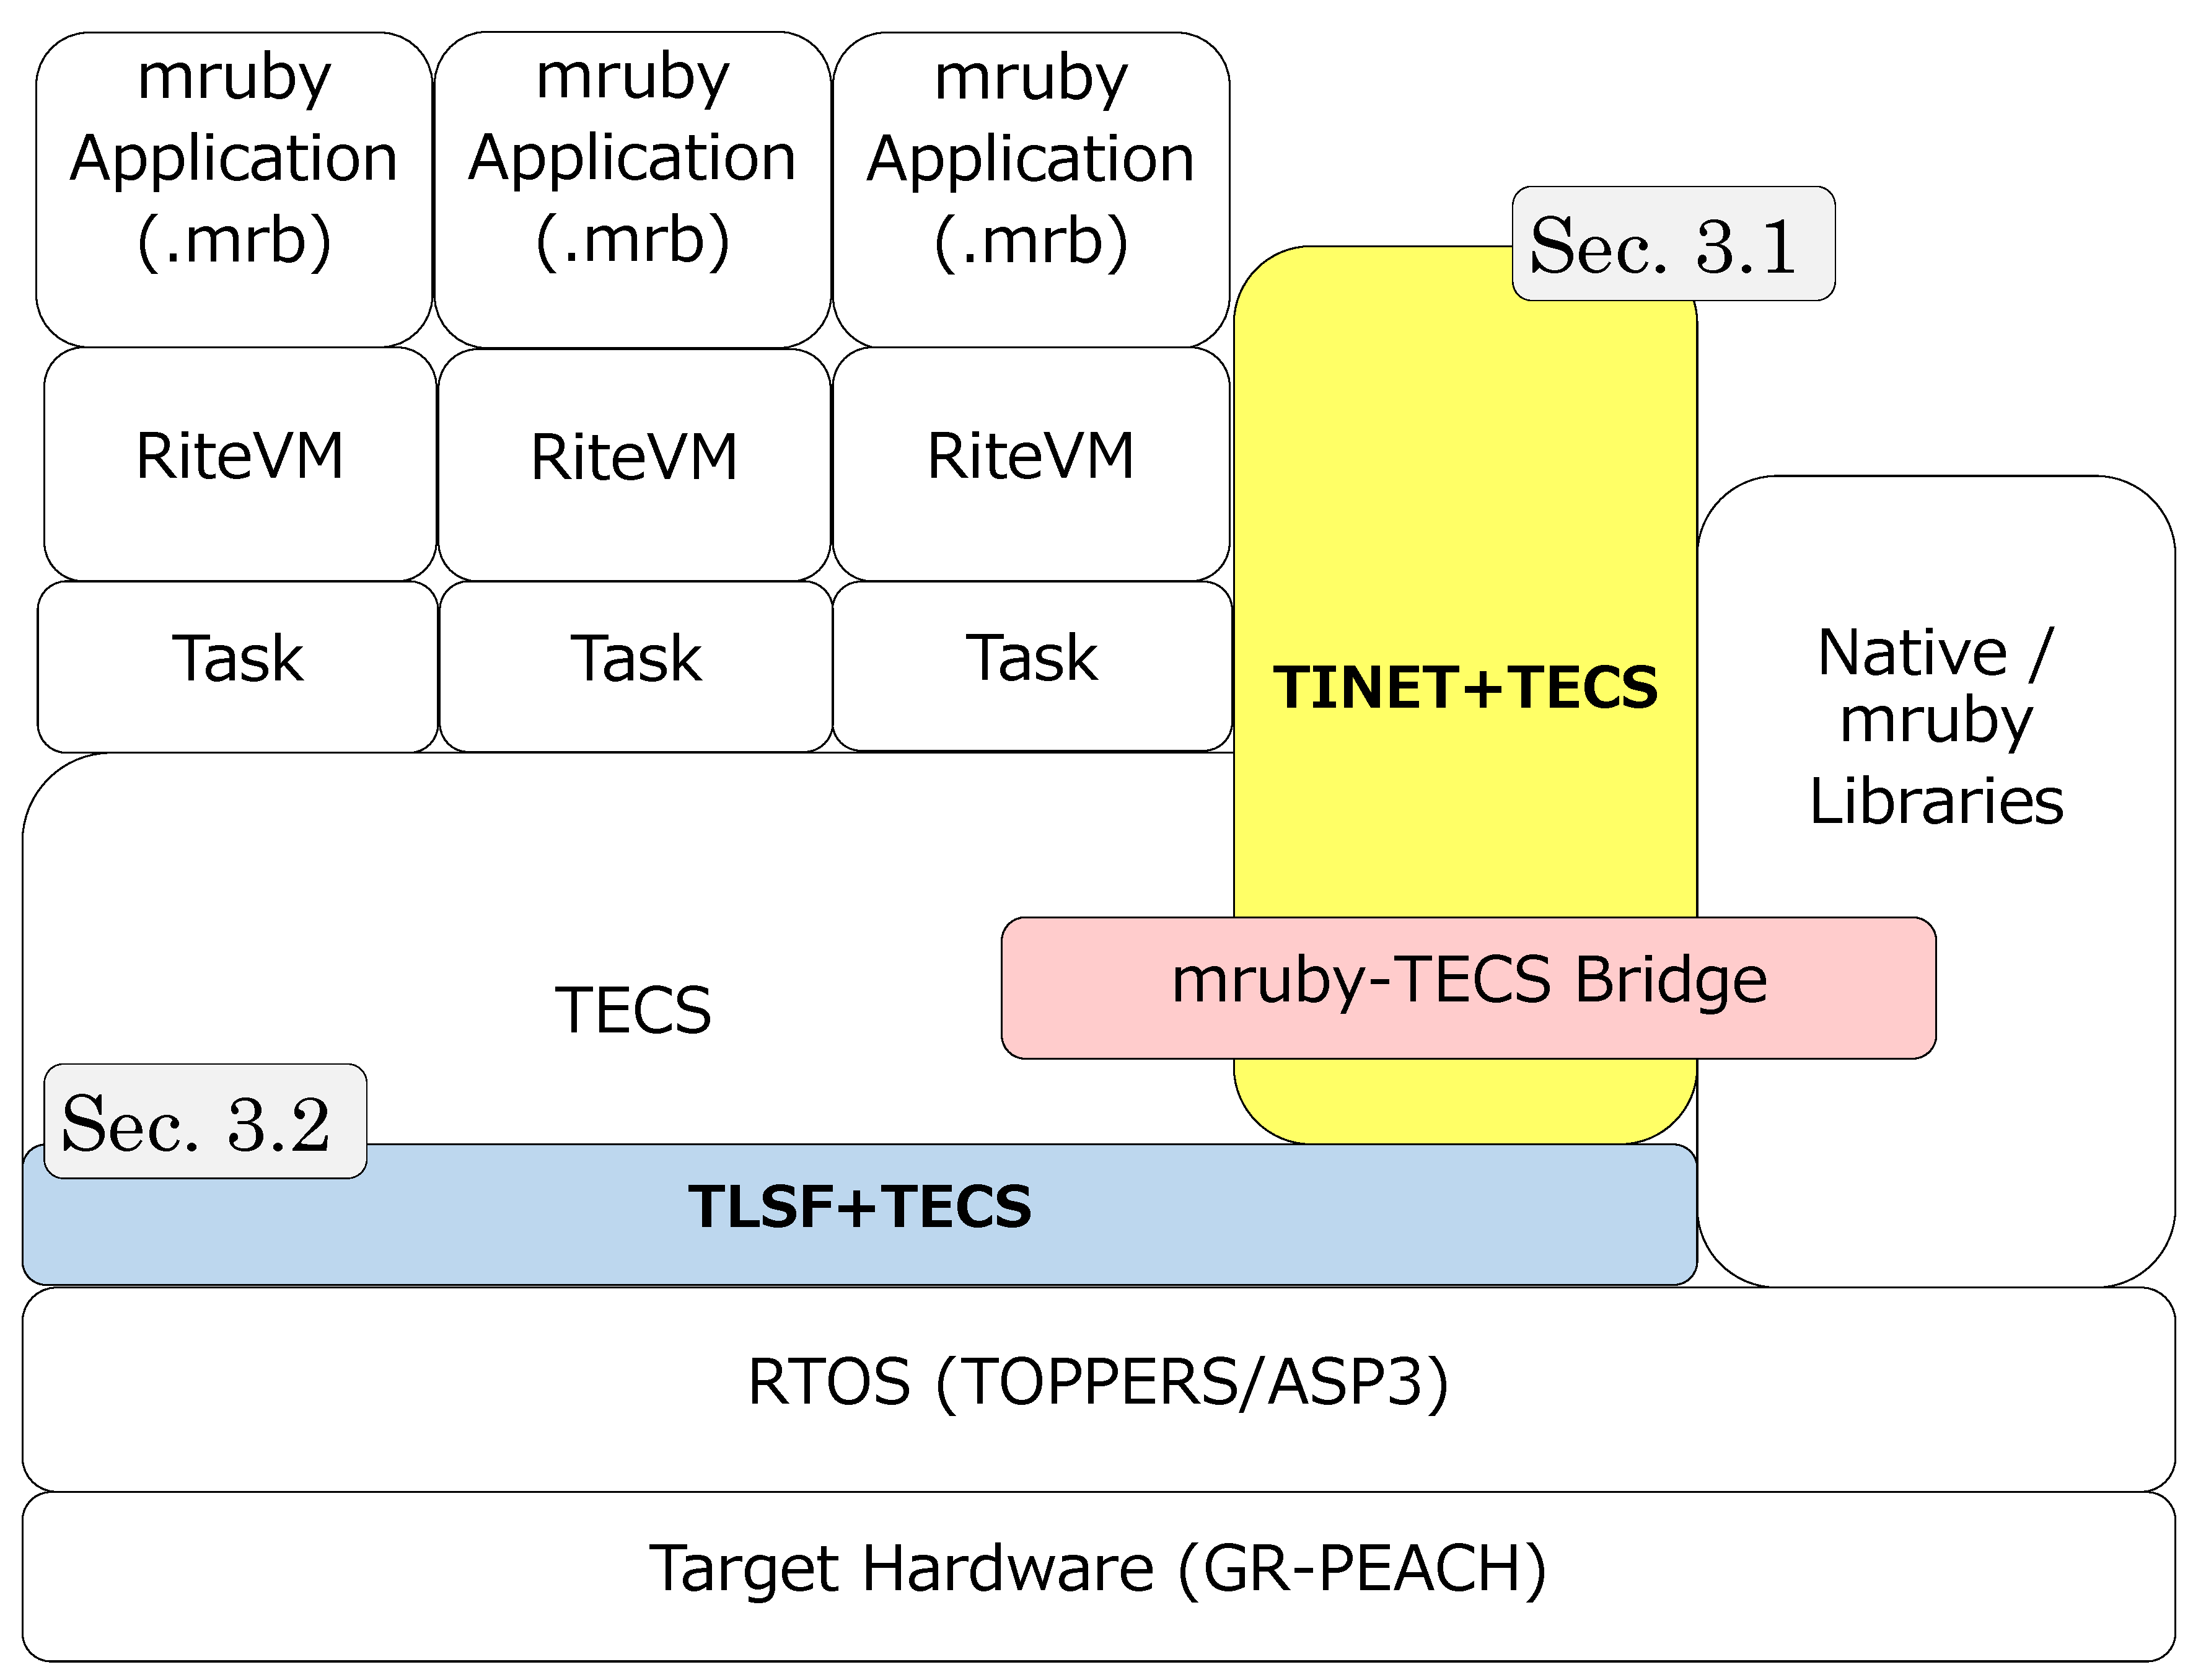
\includegraphics[width=8.0cm,clip]{figure/SystemModel.pdf}
    \caption{System model of the proposed framework}
    \label{fig:SystemModel}
\end{figure}

\subsection{TECS}
\label{sec:TECS}

TECS is a component system suitable for embedded systems.
TECS can increase productivity and reduce development costs due to improved reusability of software components.
TECS also provides component diagrams, which help developers visualize the overall structure of a system.

In TECS, component deployment and composition are performed statically.
Consequently, connecting components does not incur significant overhead and memory requirements can be reduced.
TECS can be implemented in C, and demonstrates various feature such as source level portability and fine-grained components.

\begin{figure}[t]
    \centering
    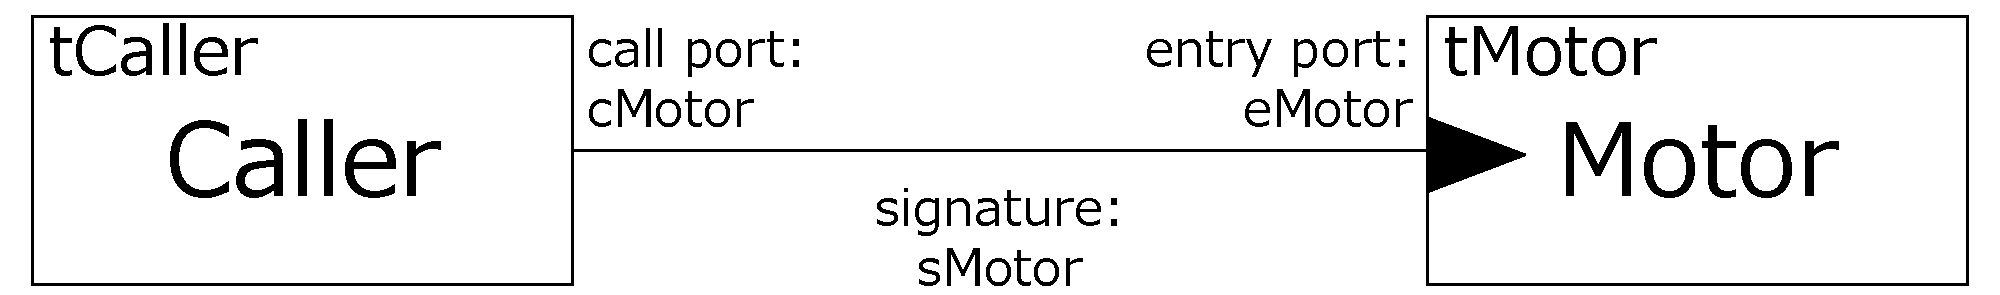
\includegraphics[width=6.5cm,clip]{figure/component_diagram.pdf}
    \caption{Component Diagram}
    \label{fig:component}
\end{figure}

\subsubsection{Component Model}
Fig.\ref{fig:component} shows a component diagram.
A {\it cell}, which is an instance of a component in TECS, consists of {\it entry} ports, {\it call} ports, attributes and internal variables.
An {\it entry} port is an interface that provides functions to other {\it cell}s, and a {\it call} port is an interface that enables the use of other {\it cell}'s functions.
A {\it cell} has one or more {\it entry} ports and {\it call} ports.
{\it Cell} functions are implemented in C.

The type of {\it entry}/{\it call} port is defined by a {\it signature}, which is a set of functions.
A {\it signature} is the interface definition of a {\it cell}.
The {\it cell}'s  {\it call} port can be connected to the {\it entry} port of another {\it cell} by the same {\it signature}.
Here, {\it celltype} defines one or more {\it call}/{\it entry} ports, attributes, and internal variables of a {\it cell}.


\subsubsection{Component Description}
In TECS, components are described by {\it signature}, {\it celltype}, and build written in component description language (CDL).
% TECS code is written in CDL (component description language) file.
These components are described as follows.

\begin{description}
    \item[{\bf Signature Description}]\mbox{}\\
        The {\it signature} defines a {\it cell} interface.
        The {\it signature} name follows the keyword {\it signature} and takes the prefix ``s'' e.g., sMotor (Fig.\ref{signature}).
        In TECS, to clarify the function of an interface, specifiers such as [in] and [out] are used, which represent input and output, respectively.
\begin{figure}[t]
\centering
\begin{lstlisting}
signature sMotor {
    int32_t getCounts( void );
    ER resetCounts( void );
    ER setPower( [in]int power );
    ER stop( [in] bool_t brake );
    ER rotate( [in] int degrees,
               [in] uint32_t speed_abs,
                [in] bool_t blocking );
    void initializePort( [in]int32_t type );
};
\end{lstlisting}
\caption{Signature Description}
\label{signature}
\end{figure}
    \item[{\bf Celltype Description}]\mbox{}\\
        The {\it celltype} defines {\it entry} ports, {\it call} ports, attributes, and variables.
        A {\it celltype} name with the prefix ``t'' follows the keyword {\it celltype}, e.g., tCaller (Fig.\ref{celltype}).
        To define {\it entry} ports, a {\it signature}, e.g., sMotor, and an {\it entry} port name, e.g., eMotor, follow the keyword {\it entry}.
        {\it Call} ports are defined similarly.
        Attributes and variables follow the keywords {\it attr} and {\it var}, respectively.
\begin{figure}[t]
\centering
\begin{lstlisting}
celltype tCaller {
    call sMotor cMotor;
};
celltype tMotor {
    entry sMotor eMotor;
    attr {
        int32_t port;
    };
    var {
        int32_t currentSpeed = 0;
    };
};
\end{lstlisting}
\caption{Celltype Description}
\label{celltype}
\end{figure}
    \item[{\bf Build Description}]\mbox{}\\
        The build description is used to instantiate and connect {\it cell}s.
        Fig.\ref{build} shows an example of a build description.
        A {\it celltype} name and {\it cell} name, e.g., tMotor and Motor, respectively, follow the keyword {\it cell}.
        To compose {\it cell}s, a {\it call} port, {\it cell}'s name, and an {\it entry} port are described in that order.
        In Fig.\ref{build}, {\it entry} port eMotor in {\it cell} Motor is connected to {\it call} port cMotor in {\it cell} Caller.
        {\it C\_EXP} calls macros defined in C files.

\begin{figure}[t]
\centering
\begin{lstlisting}
cell tMotor Motor {
    port = C_EXP("PORT_A");
};
cell tCaller Caller {
    cMotor = Motor.eMotor;
};
\end{lstlisting}
\caption{Build Description}
\label{build}
\end{figure}

\end{description}

\subsubsection{Development Flow}

\begin{figure}[t]
    \centering
    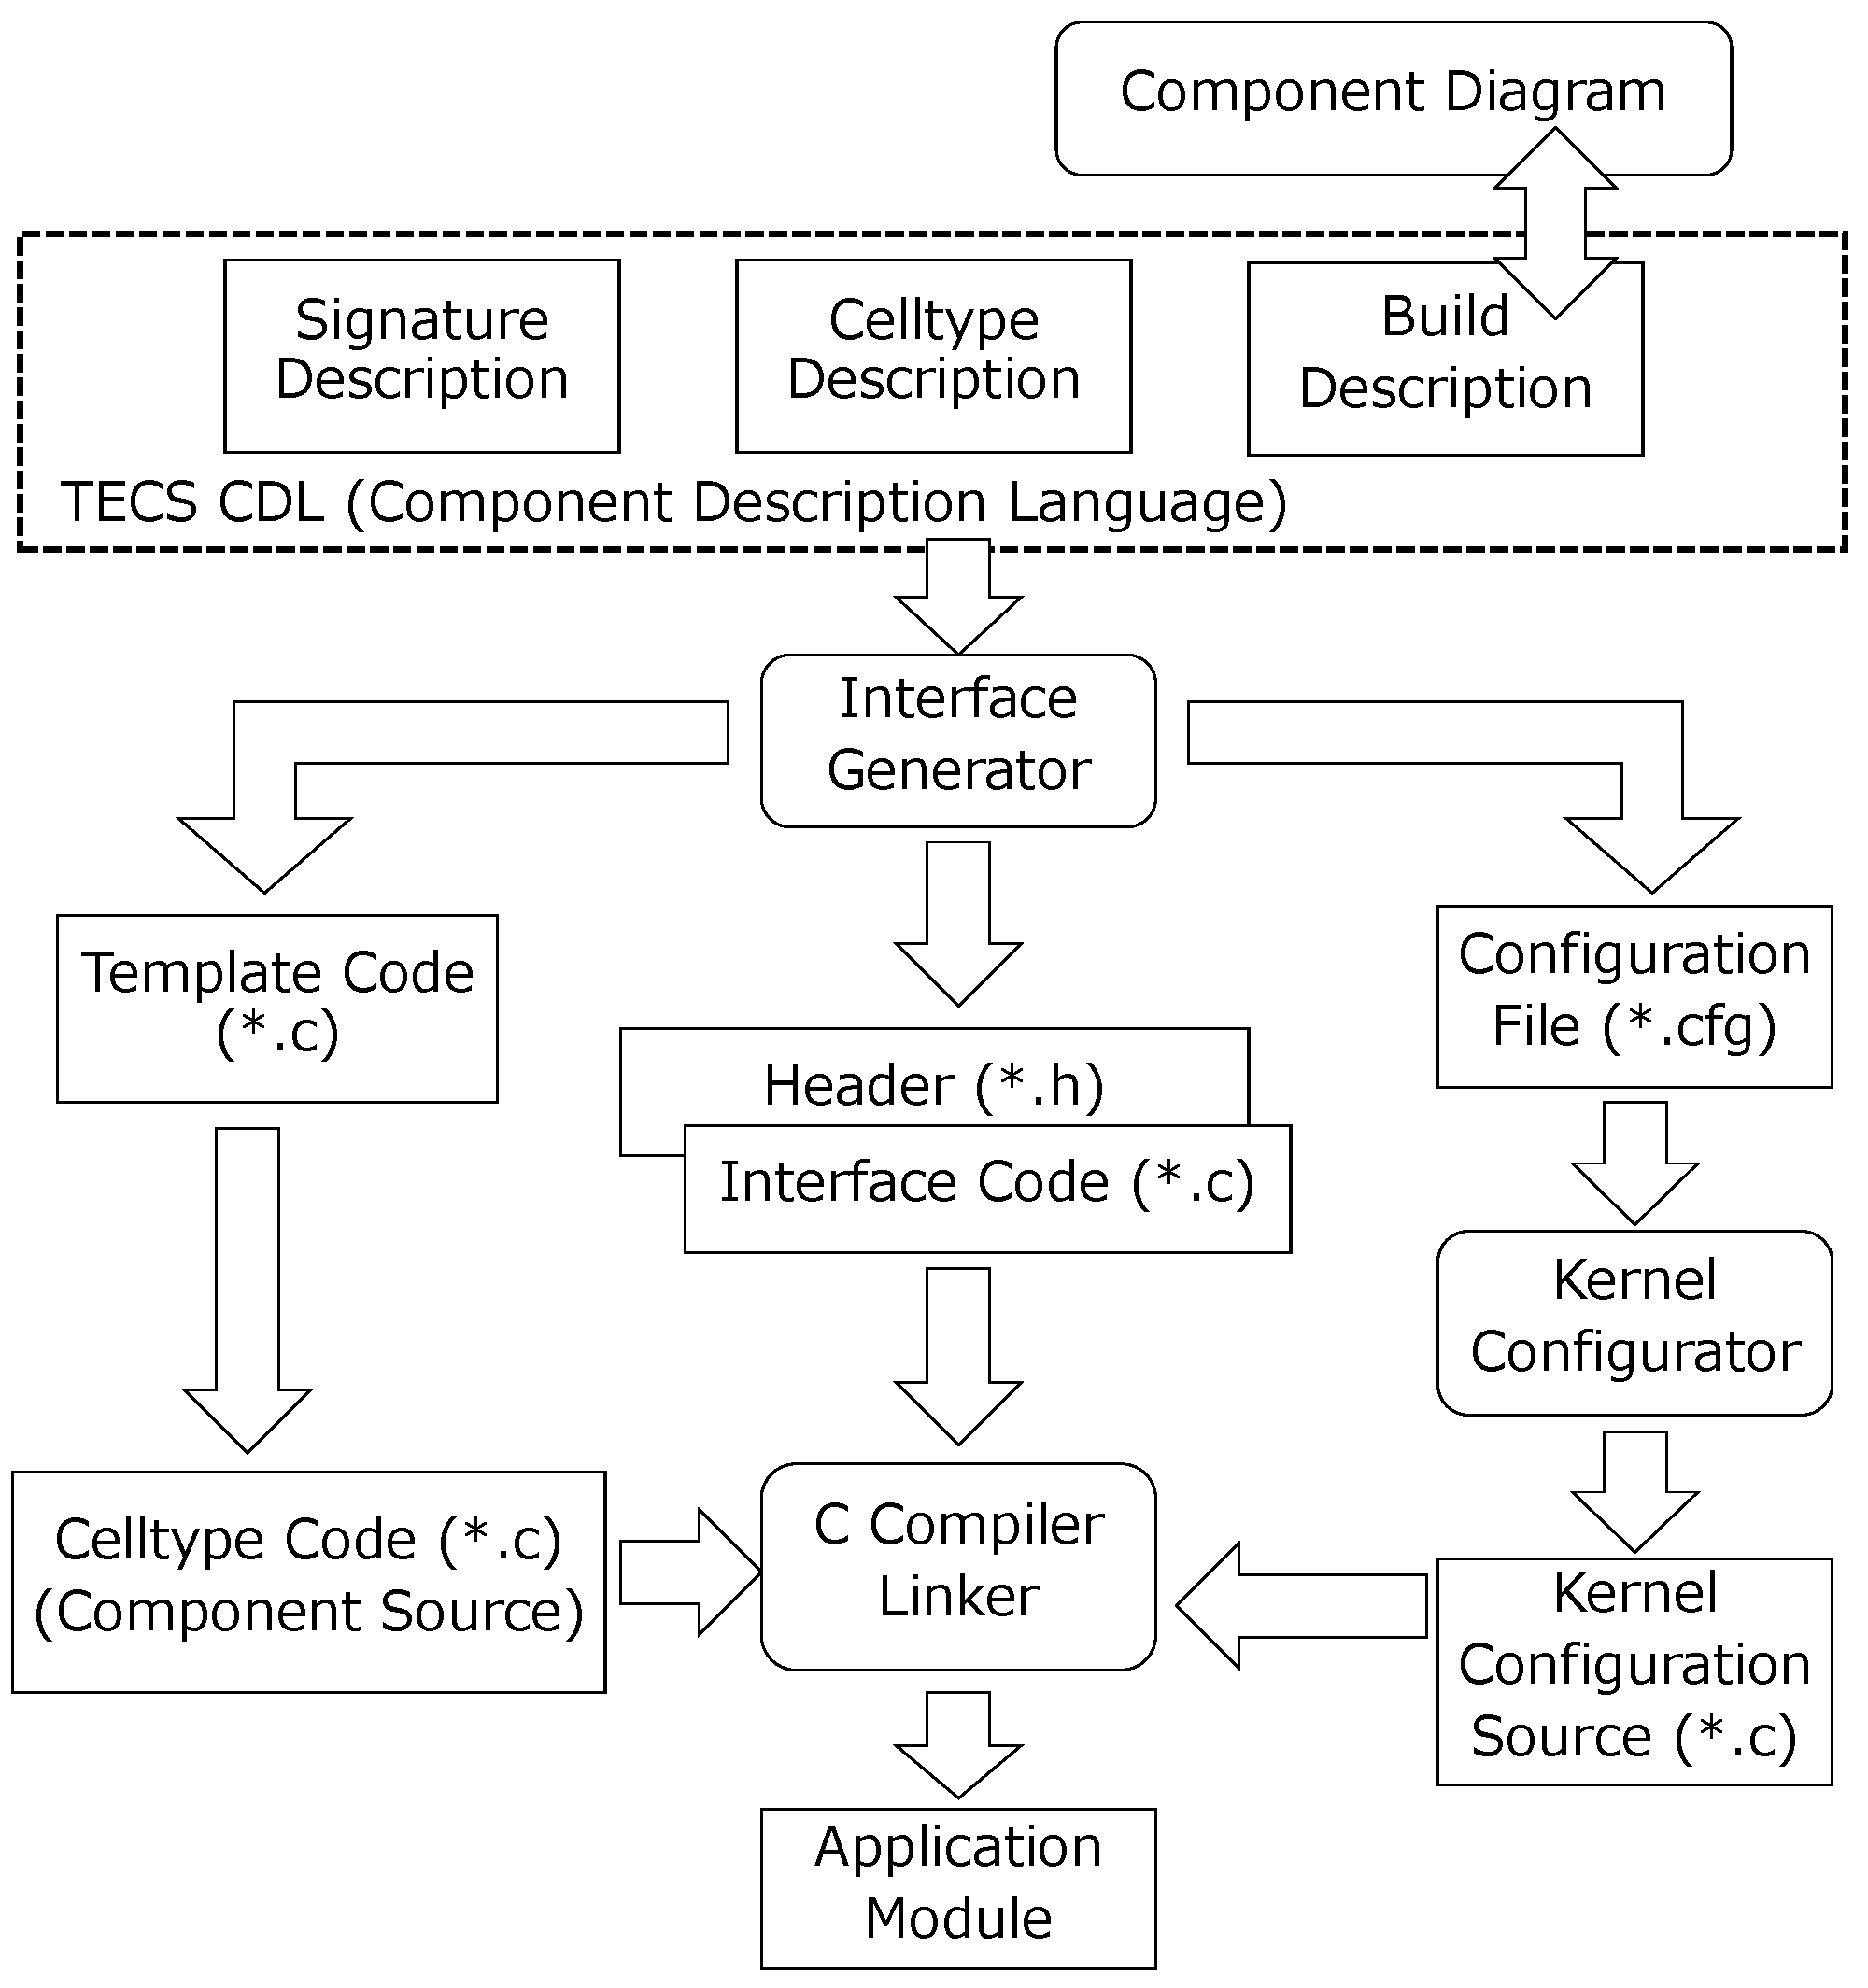
\includegraphics[width=8cm,clip]{figure/TECSFlow.pdf}
    \caption{Development flow using TECS}
    \label{fig:TECSFlow}
\end{figure}

Fig.\ref{fig:TECSFlow} shows the development flow using TECS.
TECS generator generates the interface code (.H and .C) and the configure file of the RTOS (.cfg) from the CDL file.

Software developers using TECS can be divided into component designers and application developers.
Component designers define {\it signature}s, which are interfaces between {\it cell}s, and {\it celltype}s, which are types of {\it cell}s.
Using the template code generated from the CDL file in which these are defined, component designers implement the functions and behaviors of the component in C language.
The source code implementing the function of the component is called a {\it celltype} code.
Application developers develop applications by using component diagrams and predefined {\it celltype} to connect {\it cell}s with build description.
An application module is generated by compiling and linking the header, the interface code, and the {\it celltype} code.


\subsection{mruby}
\label{sec:mruby}

mruby is a light-weight implementation of the Ruby programming language complying to part of the ISO standard.
Ruby is an object-oriented scripting language \cite{url:Ruby} with classes and methods, exceptions, and garbage collection functions.
It is easy to use and read due to its simple grammar and Ruby requires fewer lines of code than C.
Ruby improves the productivity of software development due to its simple grammar and object-oriented functions.

mruby, which retains the usability and readability of Ruby, requires fewer resources, and thus, is suitable for embedded systems.
In addition, mruby includes a VM mechanism, and thus, mruby programs can run on any operating system as long as a VM is implemented.
The mruby/RiteVM mechanism is shown in Fig.\ref{fig:mruby}.
The mruby compiler translates an mruby code into a bytecode, which can be interpreted by a RiteVM; thus, mruby programs can be executed on any target device with a RiteVM.

\begin{figure}[t]
    \centering
    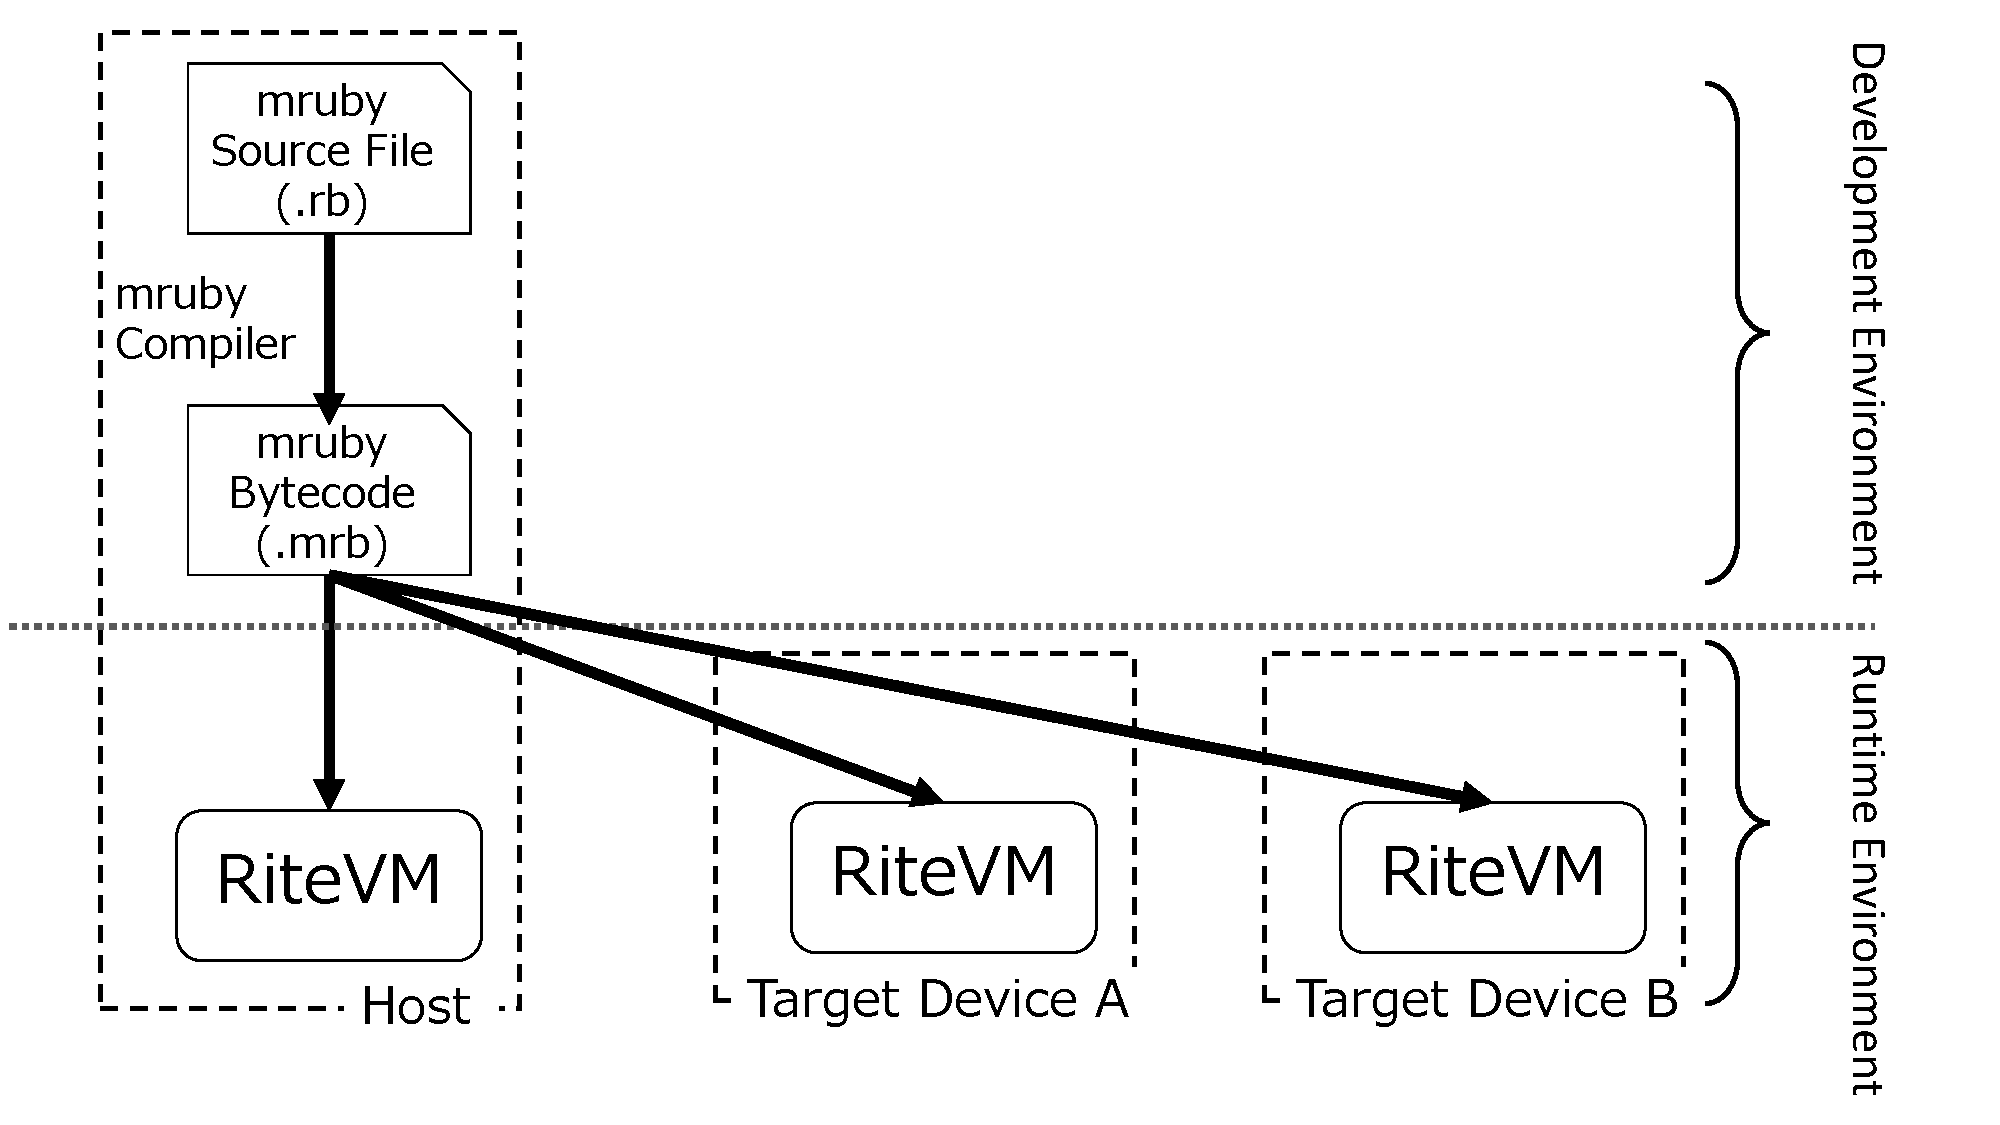
\includegraphics[width=6.5cm,clip]{figure/mruby.pdf}
    \caption{mruby/RiteVM mechanism}
    \label{fig:mruby}
\end{figure}

\subsection{mruby on TECS}
\label{sec:mrubyonTECS}

mruby on TECS is a component-based framework for running an mruby script language on embedded systems.
This framework integrates two technologies, mruby and TECS, and enables to develop embedded software using a script language without slowing down the execution time. 

\subsubsection{System Model of mruby on TECS}
The present mruby on TECS system model is shown in Fig.\ref{fig:mrubyonTECS}.
Each mruby program, which is a bytecode, runs on its own RiteVM as a componentized task of an RTOS.
TECS components support various embedded drivers such as motor and sensor drivers.

An mruby-TECS bridge provides native libraries for mruby and can call a native program (e.g., C legacy code) from an mruby program.
The mruby-TECS bridge also provides TECS components for receiving the invocation from an mruby program.

In this paper, TOPPERS/ASP3 \cite{par:ASP}, \cite{url:ASP} is the target RTOS and is based on $\mu$ITRON \cite{par:microITRON} .
However, mruby on TECS does not depend on the RTOS because TECS supports not only TOPPERS/ASP3 but also the other RTOSs such as OSEK \cite{par:OSEK} and TOPPERS/HRP2 \cite{url:HRP2}, \cite{par:hr-tecs}.

\begin{figure}[t]
    \centering
    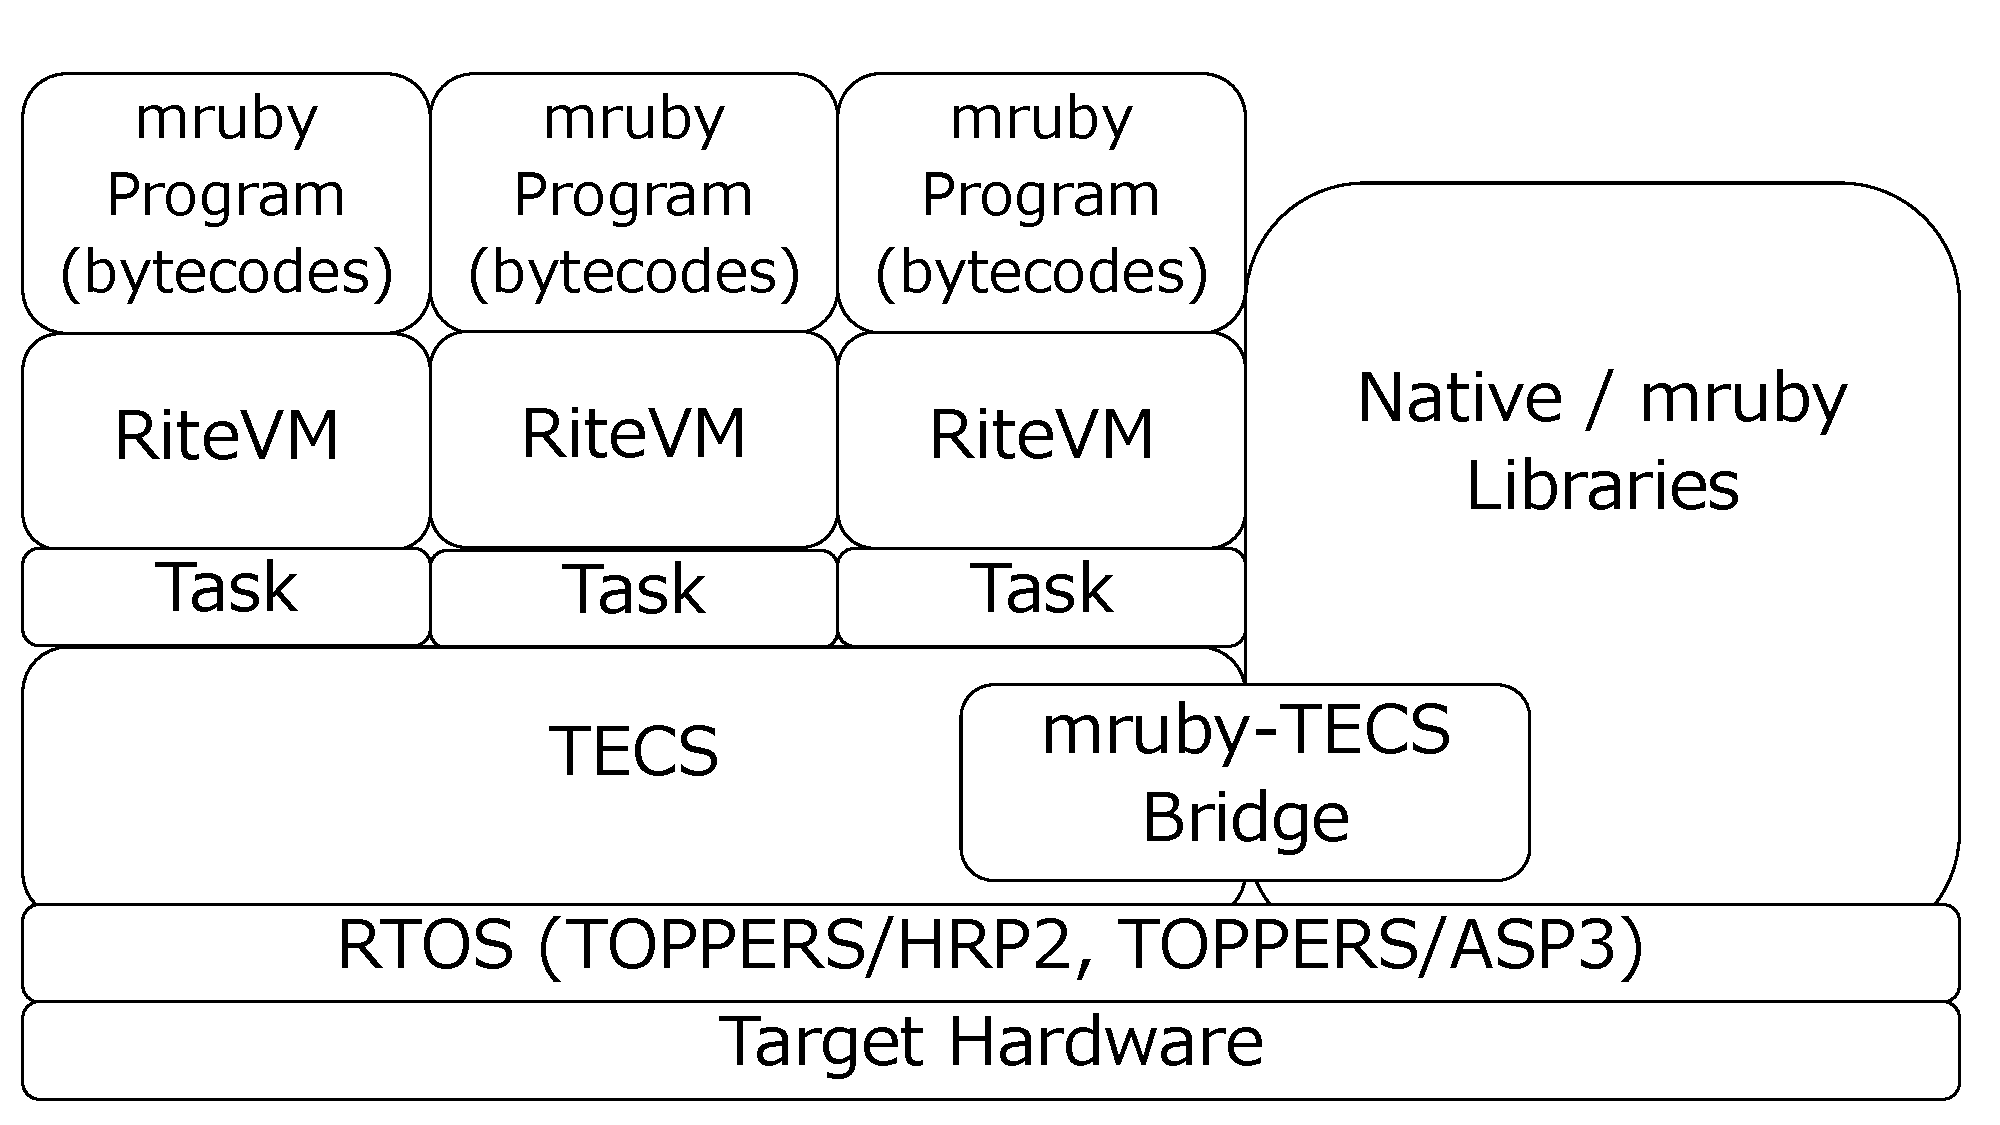
\includegraphics[width=6.5cm,clip]{figure/mrubyonTECS.pdf}
\caption{System model of existing mruby on TECS}
\label{fig:mrubyonTECS}
\end{figure}

\subsubsection{mruby-TECS Bridge}
There is a significant difference between the execution times of mruby and C language codes.
According to  \cite{par:mrubyonTECS}, mruby programs are several hundred times slower than C programs and the execution of an mruby bytecode on a RiteVM is not as efficient as that of C code.
Thus, it is difficult to use mruby exclusively.

Using Ruby on embedded devices improves productivity and maintainability because it is easy to use and read.
However, some C language codes are required to manipulate actuators and sensors and ensure that critical sections of the code run quickly.

Fig.\ref{fig:mrubyTECSbridge} illustrates an mruby-TECS bridge used to control a motor.
The left side of BridgeMotor belongs to the mruby program.
The right side of BridgeMotor belongs to TECS component.

\begin{figure}[t]
    \centering
    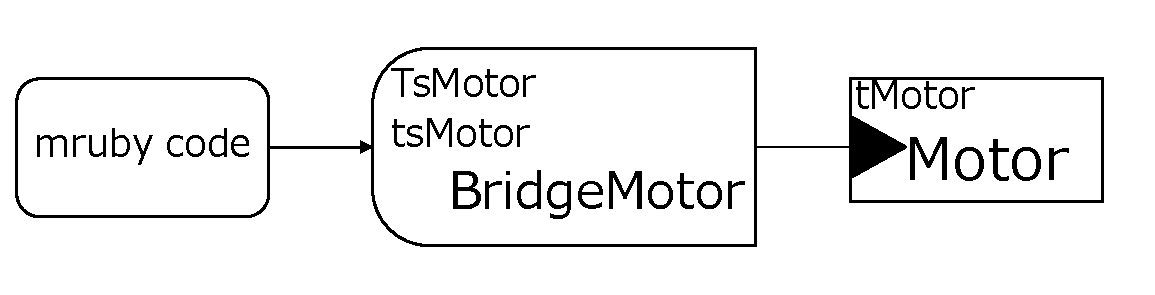
\includegraphics[width=6.5cm,clip]{figure/mrubyTECSbridge.pdf}
\caption{mruby-TECS bridge}
\label{fig:mrubyTECSbridge}
\end{figure}

The mruby-TECS bridge generates a {\it celltype}, which is called from the mruby code, and an mruby class, which corresponds to a developer-specified TECS component to invoke a C function from the mruby program.
The generated mruby-TECS bridge supports registration of classes and methods for mruby.
Methods in an mruby class are defined by generation codes for an mruby-TECS bridge, such as setPower and stop.
Thus, when a method is called in an mruby program, the mruby-TECS bridge calls the function defined in the TECS component such as a Motor {\it cell}.

%3
\section{Proposed Framework}
\label{sec:Proposed Framework}

The proposed framework is an extended mruby on TECS framework for network programming.
It can use TINET+TECS functions from mruby programs.
TINET+TECS is a component-based TCP/IP protocol stack comprised in the proposed framework, and it compensates for the original TINET's weak point, that it is hard to maintain, extend, and analyze the software due to many complex source codes and improves the configurability.
In addition, TLSF+TECS, a component-based dynamic memory allocator, is used for memory management of mruby's RiteVMs and TCP/IP buffers in the proposed framework.
Since each component holds its own heap area, TLSF+TECS allows concurrent operation without exclusive control while improving the efficiency of memory consumption which is a merit of TLSF.


\subsection{TINET+TECS}
\label{sec:TINET+TECS}

\subsubsection{TINET}

TINET is a compact TCP/IP protocol stack for embedded systems based on the ITRON\footnote{ITRON is a real-time operating system (RTOS) developed by the TRON project.} TCP/IP API Specification \cite{url:ITRON_TCP/IP_API_Spec}, developed by the TOPPERS Project \cite{url:TOPPERS}.
TINET has been released as an open-source tool.

To satisfy restrictions for embedded systems in terms of, for example, memory capacity, size, and power consumption, TINET supports the following functions:

\begin{itemize}
    \item minimum copy frequency,
    \item elimination of dynamic memory control,
    \item asynchronous interfacing,
    \item error detailing per API.
\end{itemize}

{\bf Overview:}
TINET runs as middleware on TOPPERS/ASP3 \cite{par:ASP3} \cite{url:ASP3}, a real-time kernel based on $\mu$ITRON \cite{par:microITRON}.
As it is compatible with TOPPERS RTOS, TINET also supports other RTOSs such as TOPPERS/ASP and TOPPERS/JSP.

Fig.\ref{fig:TINETHierarchyDiagram} shows the hierarchy diagram of TINET and TOPPERS/ASP3.
Users transmit and receive data using a Communication End Point (CEP), an interface that functions like a socket.
In the transmission process, headers are attached to the data body passed to the CEP at each protocol layer before the data are transmitted from the network device.
In the reception process, the headers of the data bodies received by the network device are analyzed at each protocol layer, and the data are then passed to the CEP.

A TCP reception point called the REP stands by to receive connection requests from the partner side.
The REP has an IP address ({\it myaddr}) and a port number ({\it myportno}) as attributes and performs functions such {\it bind()} and {\it listen()}.

In TINET, the amount of data copying between each protocol layers is minimized.
In standard computing systems, the TCP/IP protocol stack has large overheads in terms of execution time and memory consumption because the data are copied at each protocol layer.
To solve this problem, TINET does pass the pointer of the data buffer between each protocol layer instead of performing data copying.

\begin{figure}[t]
    \centering
    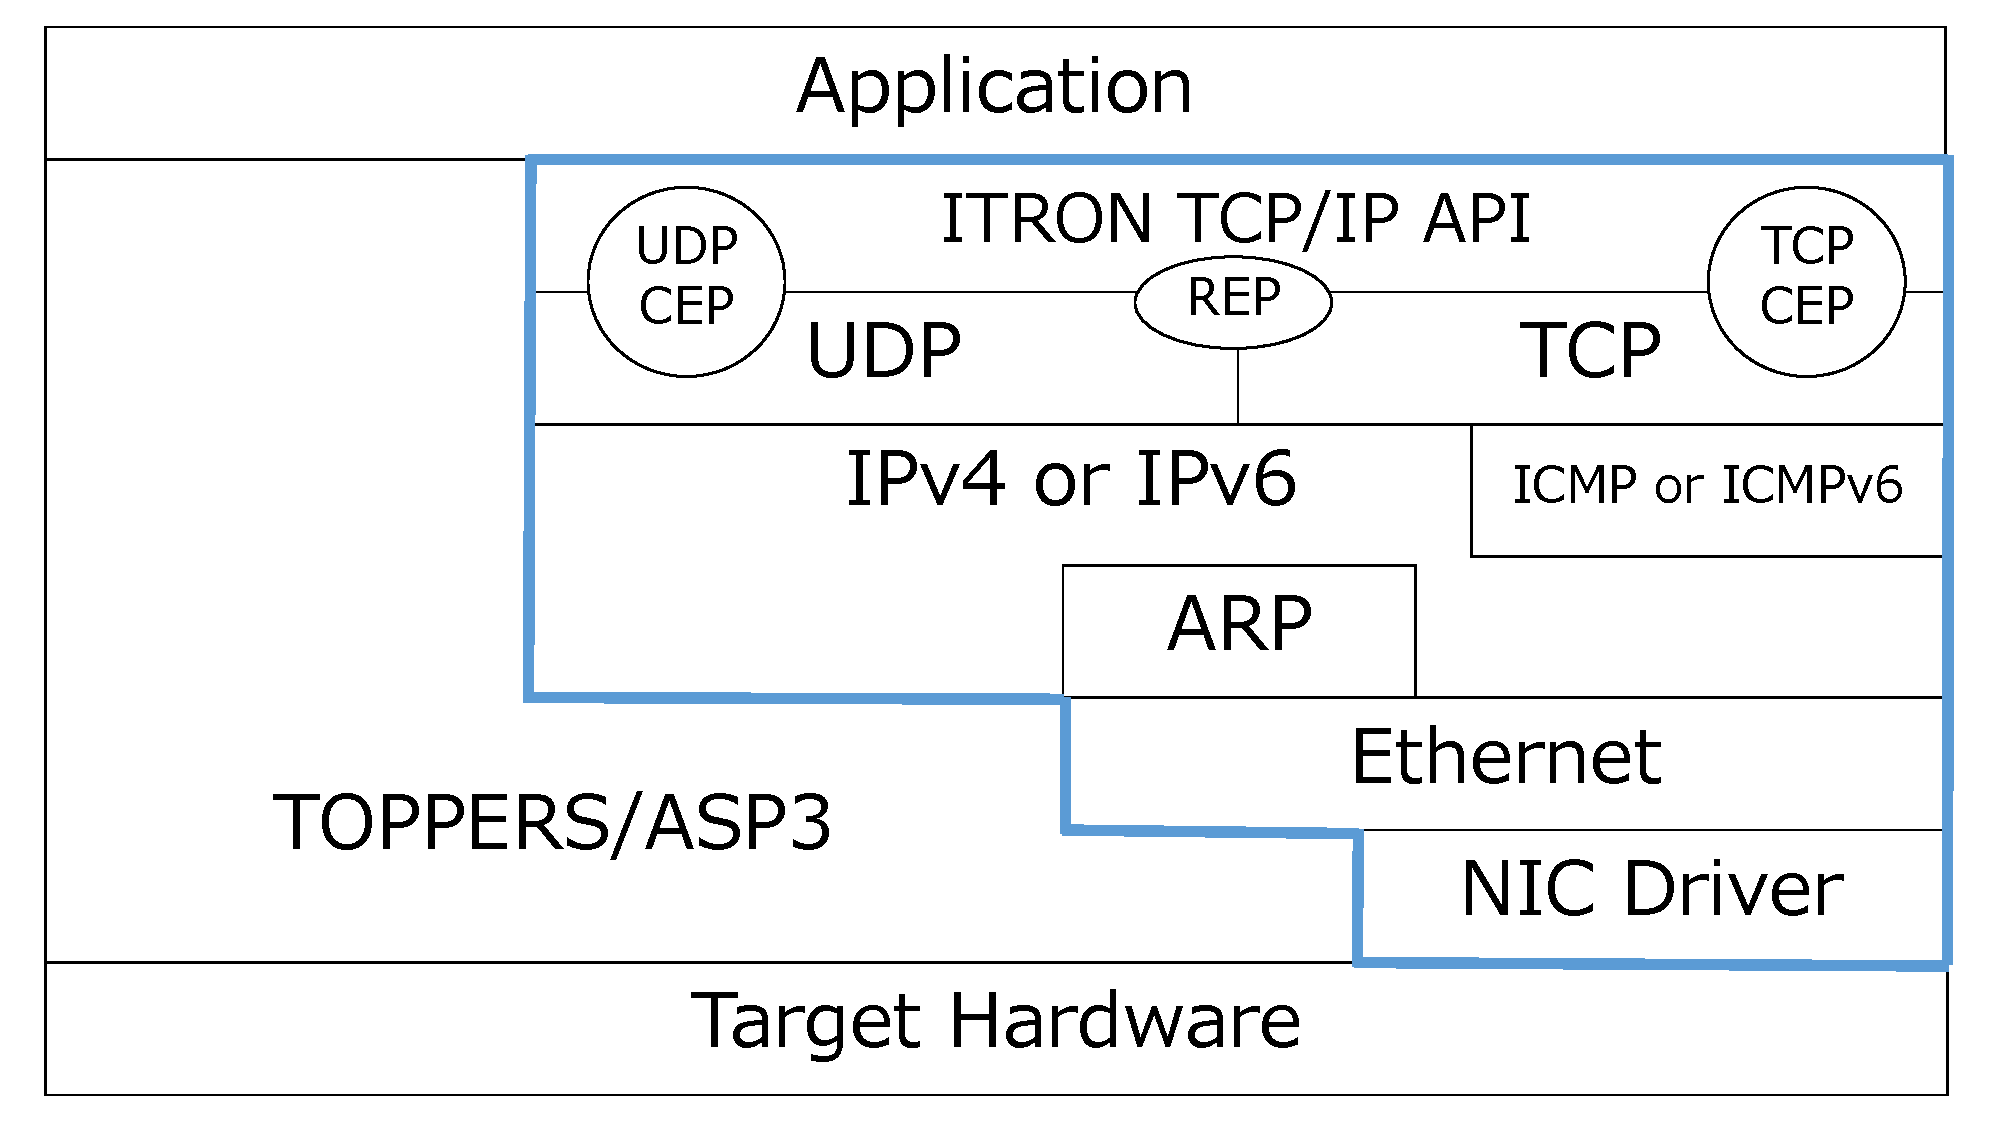
\includegraphics[width=7.0cm,clip]{figure/TINETHierarchyDiagram.pdf}
    \caption{TINET and TOPPERS/ASP3 hierarchy diagrams}
    \label{fig:TINETHierarchyDiagram}
\end{figure}

\subsubsection{Component Design of TINET+TECS}

TINET+TECS, the proposed componentized TCP/IP protocol stack, comprises a number of some TECS components.
This section describes the components of the TINET+TECS framework with the aid of component diagrams.

\subsubsection*{Components of a protocol stack}

The components of a TINET+TECS protocol stack are shown in Fig.\ref{fig:ComponentProtocolStack}.
Note that some small particle components, such as a kernel object, data queues, and semaphores, are omitted to simplify the component diagram.
In TINET+TECS, the components are divided for each protocol, and functionalities such as input and output functions are defined as respective components.
By using such small grain components, software visibility is improved.
The components of each protocol are described in the following.

\begin{figure}[t]
    \centering
    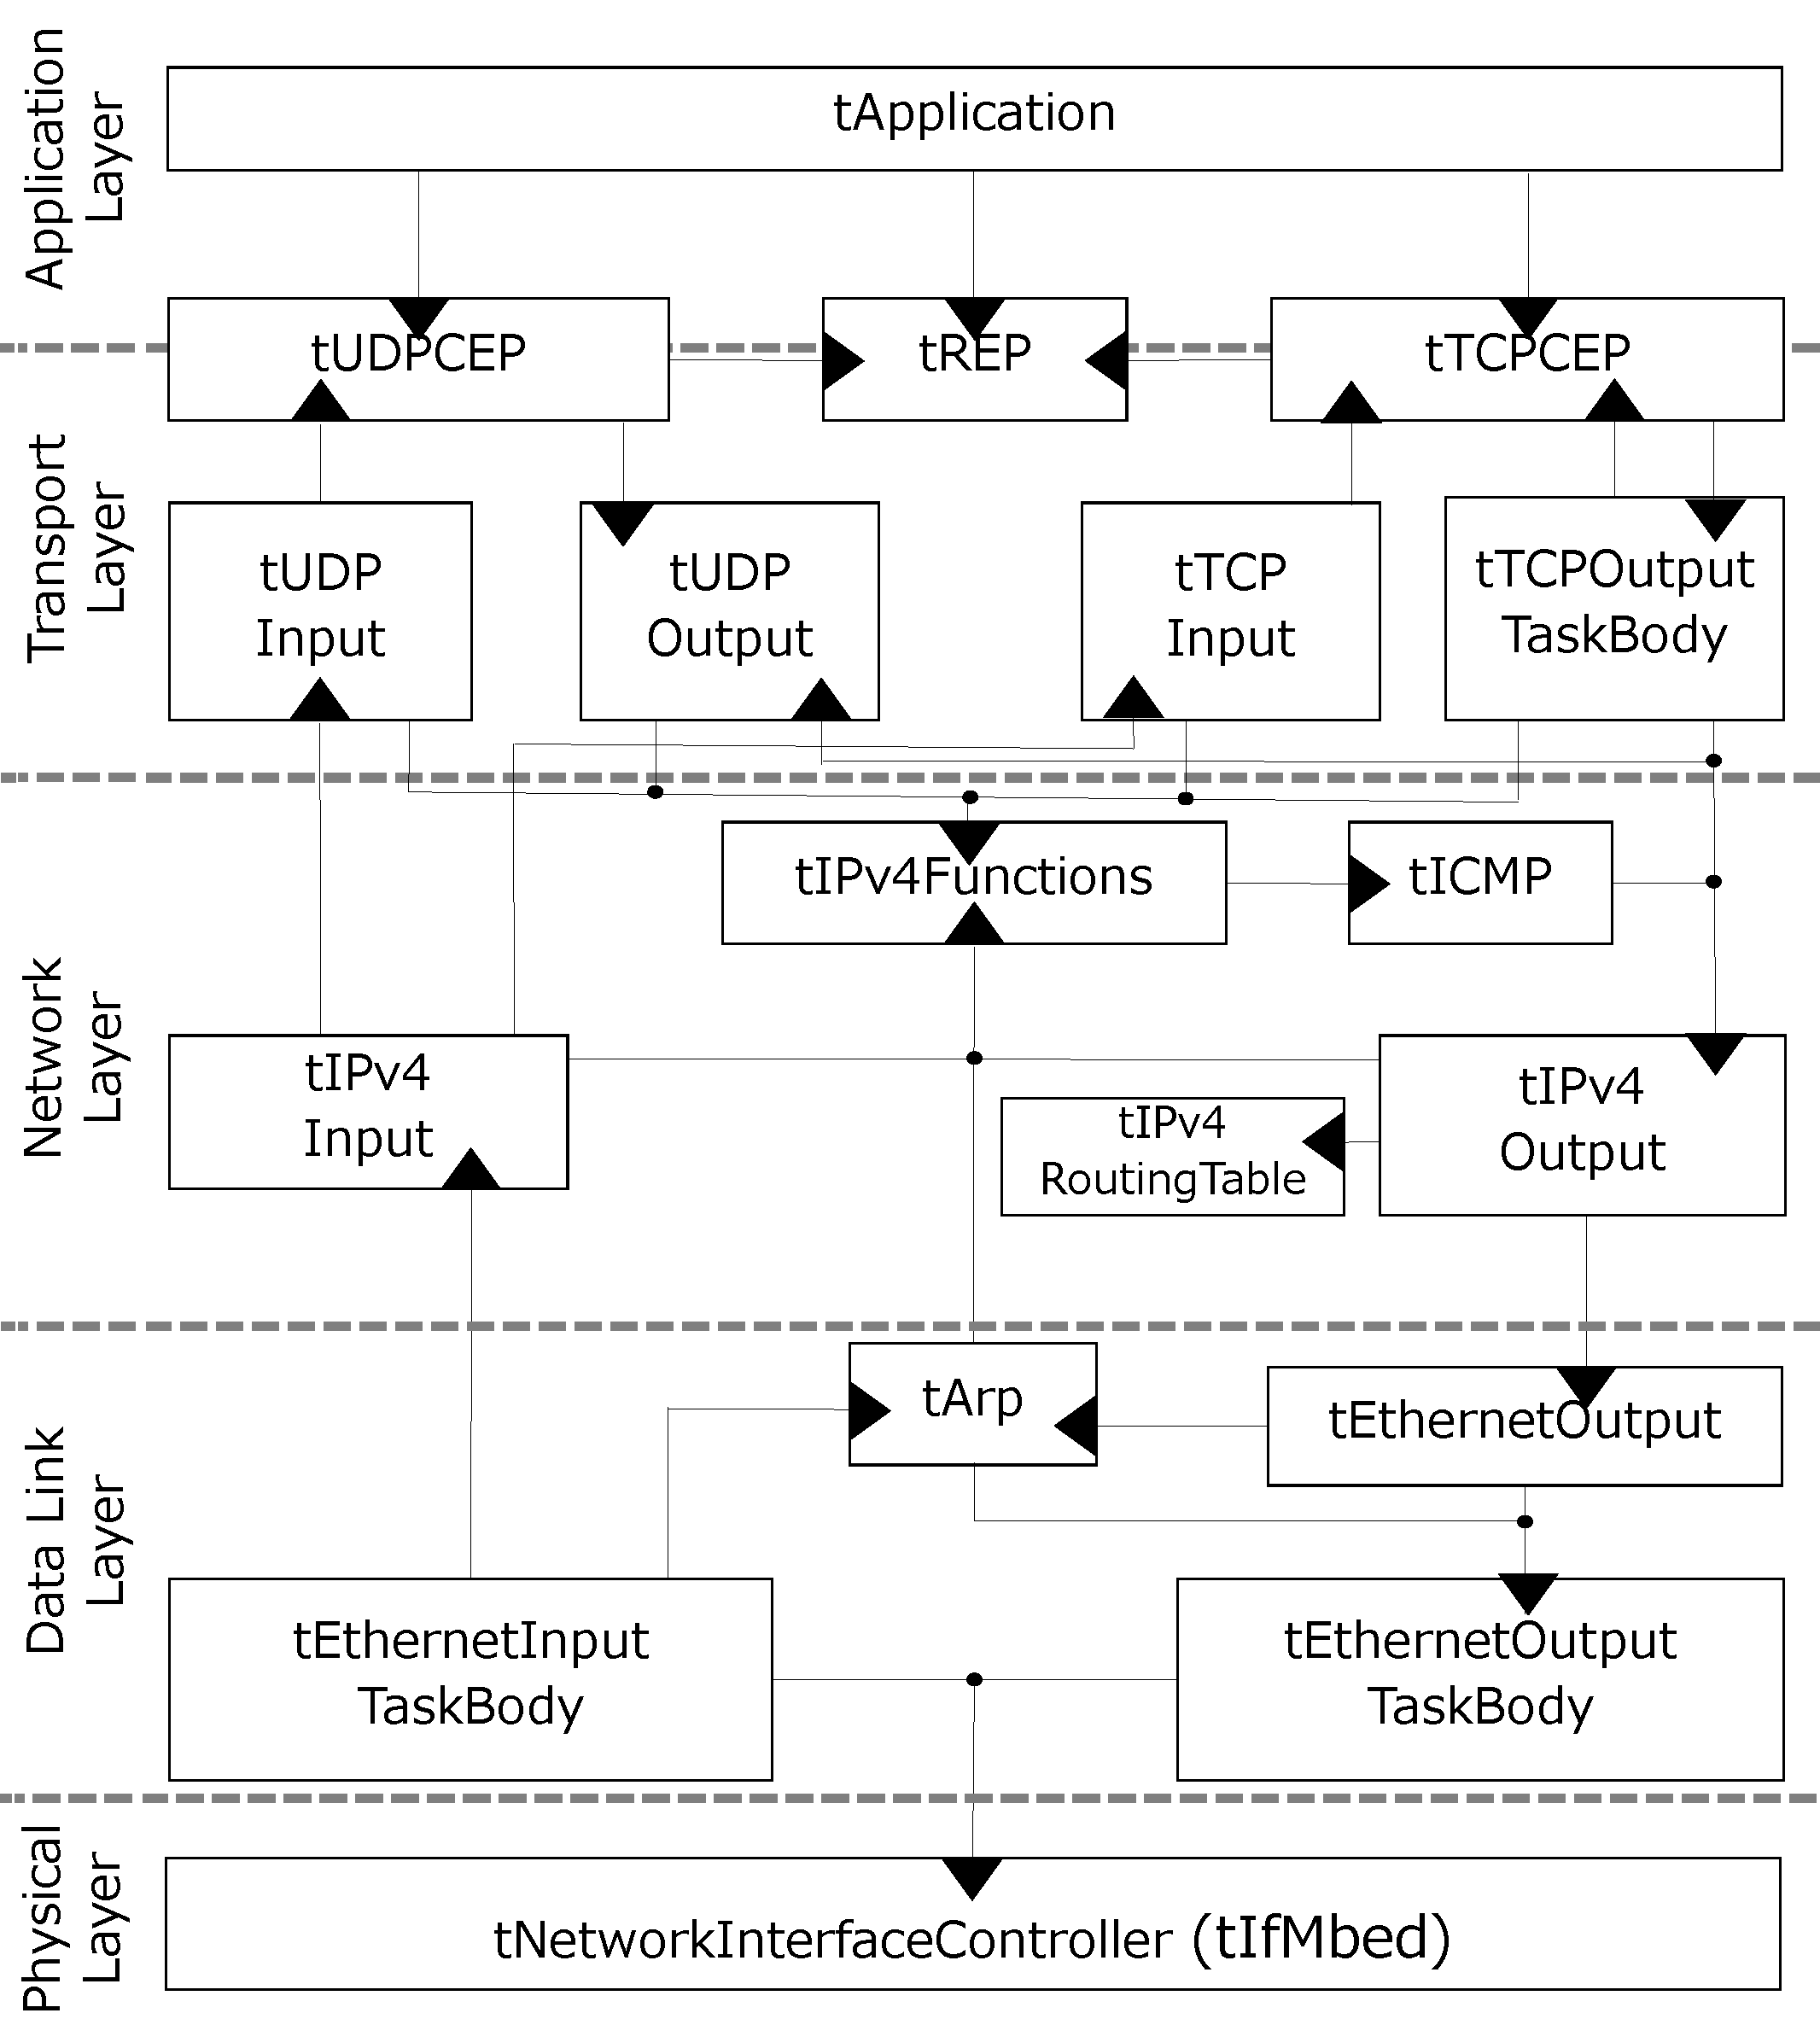
\includegraphics[width=8.0cm,clip]{figure/ComponentProtocolStack.pdf}
    \caption{Component diagram of a protocol stack}
    \label{fig:ComponentProtocolStack}
\end{figure}


{\bf Application layer:}
An application in TINET+TECS is implemented as a component such as tApplication.
Software with TINET uses ITRON TCP/IP API \cite{url:ITRON_TCP/IP_API_Spec} such as {\it tcp\_snd\_dat} and {\it tcp\_rcv\_dat}.
In TINET+TECS, the application component calls TECS functions such as {\it cTCPAPI\_sendData} and {\it cTCPAPI\_receiveData}.
Moreover, in TINET+TECS supporting a TECS adapter, an existing application with TINET can run on the TINET+TECS framework without transporting, and therefore, software can be developed either using existing methods or as TECS components.

{\bf Transport layer:}
tTCPCEP (tUDPCEP) and tREP are, respectively, CEP and REP components TCP (UDP).
For example, a server program supporting multiple clients can be developed by preparing multiple tTCPCEP components.
tTCPInput (tUDPInput) and tTCPOutput (tUDPOutput) are components for performing, respectively, receiving and sending processing in the transport layer.

{\bf Network layer:}
The tIPv4Input and tIPv4Output components perform, respectively, the receiving and sending processing in the network layer.
The tIPv4Functions component performs functions such as checksum, the tICMP component is used for the Internet Control Message Protocol (ICMP), and the tIPv4RoutingTable component operates a routing table.

{\bf Data link layer:}
tEthernetInputTaskBody and tEthernetOutputTaskBody (tEthernetOutput) are components for performing, respectively, receiving and sending processing in the data link layer.
The tArp component is for implementing the Address Resolution Protocol (ARP).

{\bf Physical layer:}
The tNetworkInterfaceContoroller component implements a network device driver.
Software can be run on other devices by replacing the component because only the component depends on the target device.

To utilize the protocol stack in the same manner in the original TINET, communication object components such as tTCPCEP, tUDPCEP, and tREP are defined as an interface between TINET+TECS and an application.
The communication object component corresponds to a CEP or REP of the original TINET.
Application developers can utilize the TINET+TECS functionalities by generating and combining as many components as necessary.

The protocol stack of TINET+TECS supports the coexistence of multiple protocols.
Though its use of IPv6 and Point-to-Point Protocol (PPP) components, TINET+TECS can make IPv4 and IPv6 coexist and support PPP without modification of component implementation.

\subsubsection*{Memory allocator component} 

The original TINET eliminates dynamic memory control to meet the severe memory restrictions of embedded systems.
A memory area for sending/receiving data in the protocol stack is allocated and released within a predetermined area.
The memory allocator component allows for elimination of dynamic memory control in TINET+TECS by providing a requested memory area from the statically allocated memory area.

The memory allocator component connects to as many tFixedSizeMemoryPool as required, as shown in Fig.\ref{fig:tMemoryAllocator}.
tFixedSizeMemoryPool is a componentized kernel object of TOPPERS/ASP3 for allocating and releasing memory areas of a requested size. 
tFixedSizeMemoryPool components of various sizes are prepared, and an appropriate memory area can be allocated according to the used data size.
On the other hand, all components that need to allocate or deallocate memory, e.g., tTCPInput and tEthernetOutput, connect to the memory allocator component.

In addition, TINET+TECS utilizes the TECS {\it send/receive} specifier to minimize the memory copy frequency, which is a functionality supported by TINET.

\begin{figure}[t]
    \centering
    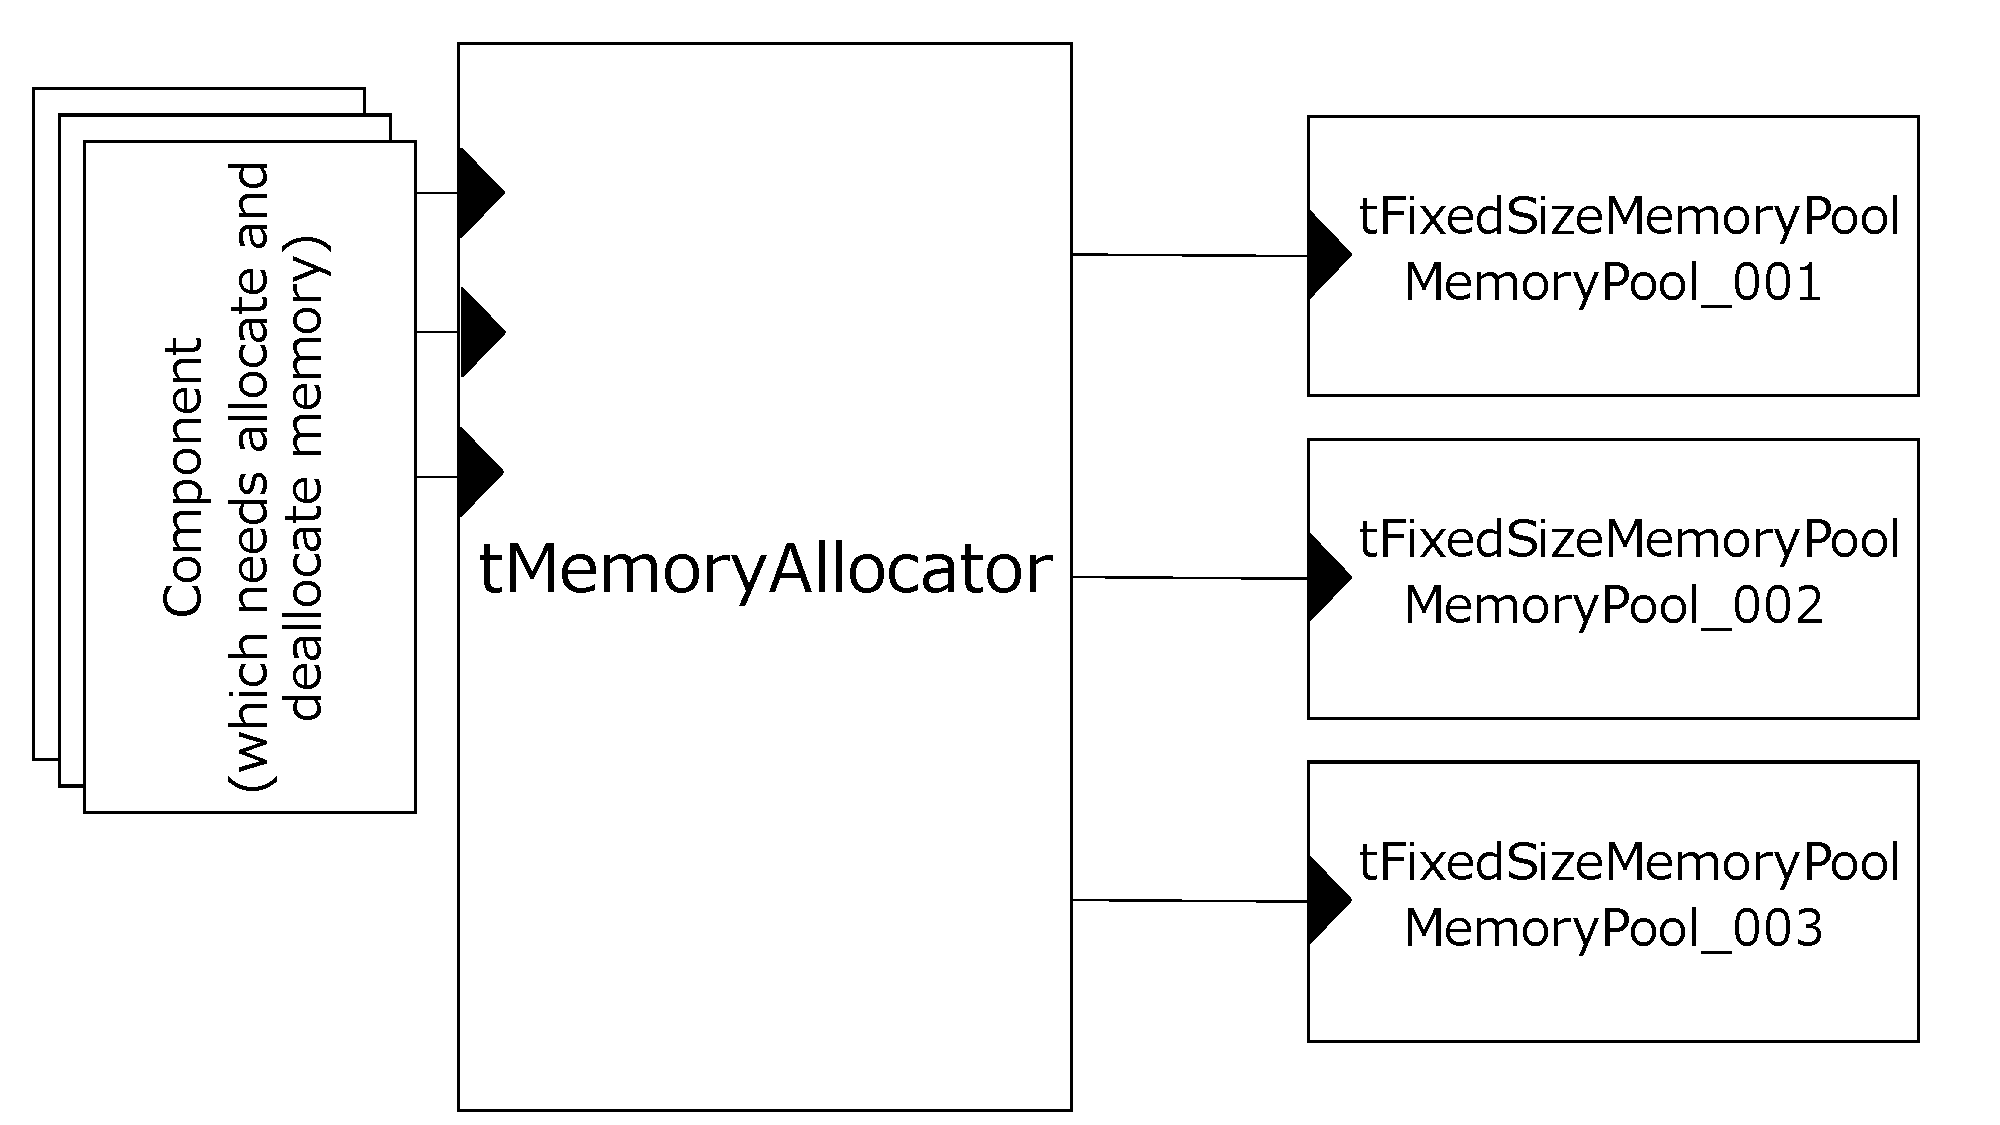
\includegraphics[width=7.0cm,clip]{figure/tMemoryAllocator.pdf}
    \caption{Component diagram of tMemoryAllocator}
    \label{fig:tMemoryAllocator}
\end{figure}

\begin{figure}[t]
    \centering
    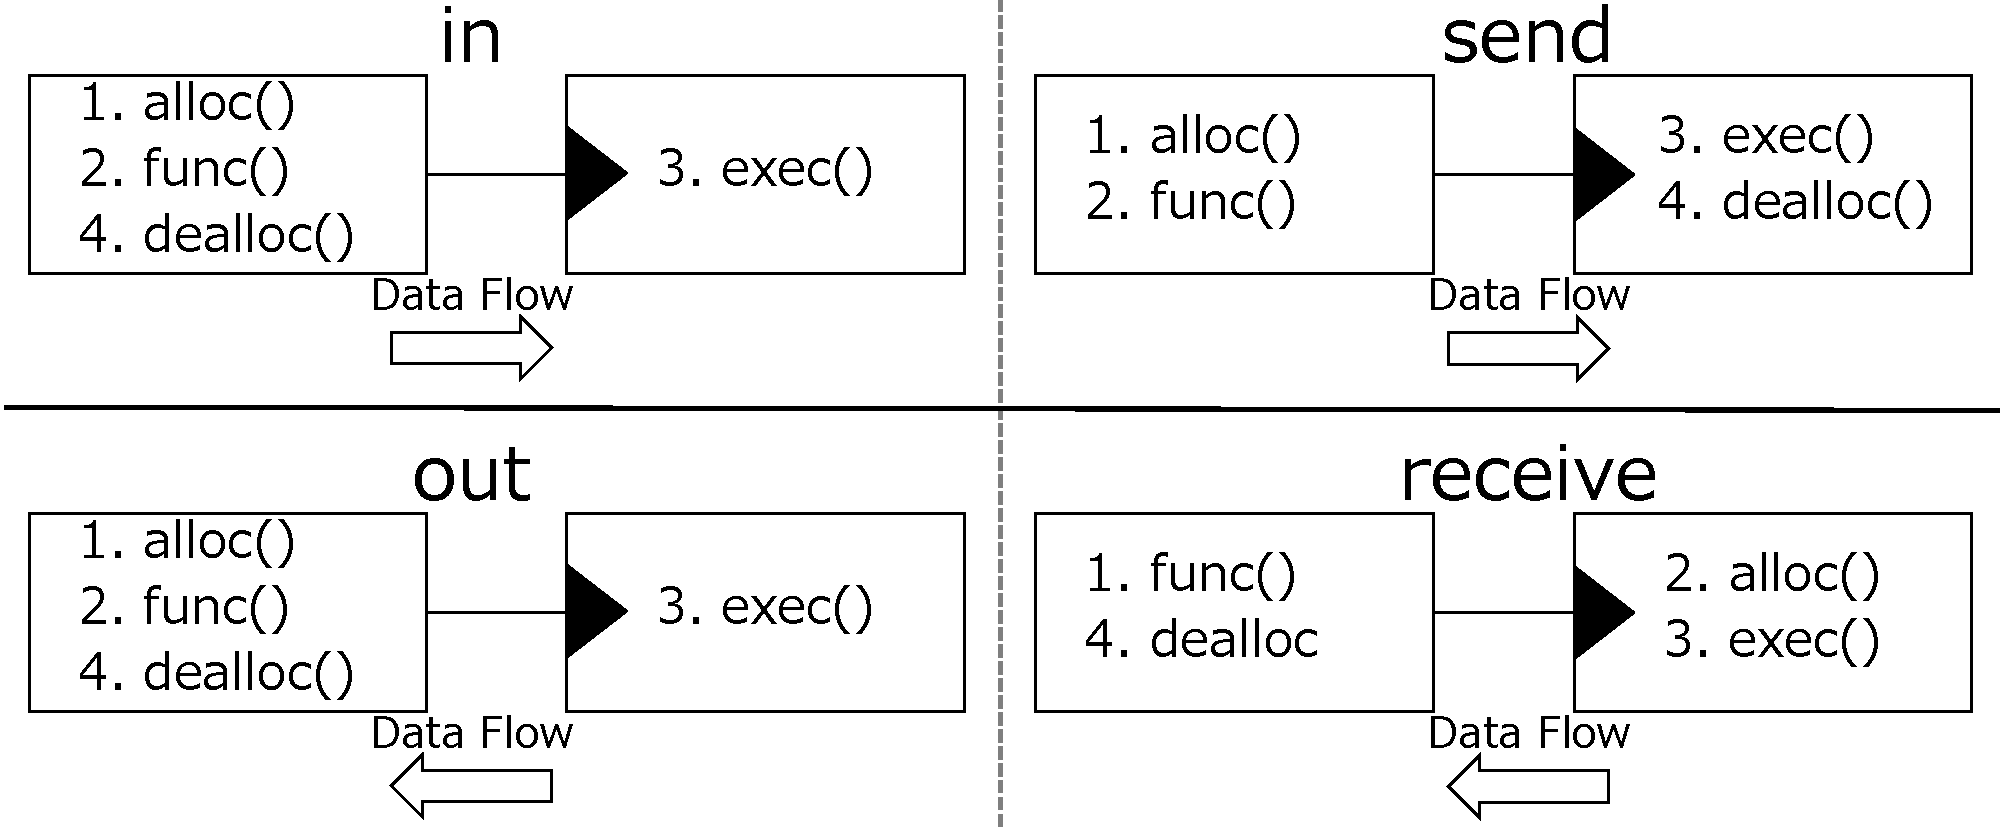
\includegraphics[width=7.0cm,clip]{figure/SendReceive.pdf}
    \caption{Differences between in/out and send/receive}
    \label{fig:SendReceive}
\end{figure}

{\bf Send/receive specifiers:}
TECS supports {\it send}/{\it receive} interface specifiers \cite{par:RPC}.
TINET+TECS uses {\it send} and {\it receive} specifiers instead of {\it in} and {\it out} to reduce the number of copies:

\begin{itemize}
\item {\it in} is a specifier for input arguments.
A callee side uses the memory of arguments with {\it in} when executing the callee function.
When the processing returns to the caller side, the caller can reuse and deallocate the memory.

\item {\it send} is another specifier for transferring data to a callee from a caller such as {\it in}.
The difference between {\it in} and {\it send} is whether the data memory is deallocated in the caller or callee, as shown in Fig.\ref{fig:SendReceive}.
In the case of the {\it in} specifier, both allocating and deallocating of the data memory are performed in the caller.
By contrast, in the case of {\it send}, the caller allocates the data memory and the callee deallocates it.

\item {\it out} is a specifier for output arguments through which a callee writes data in the memory allocated by a caller while the caller receives the data.

\item {\it receive} is another specifier for a caller receiving data from a callee such as {\it out}.
The difference between {\it out} and {\it receive} lies in whether the data memory is allocated in the caller or callee, as shown in Fig.\ref{fig:SendReceive}.
In the case of {\it out}, the callee writes data in the memory allocated by a caller, whereas in the {\it receive} case, the callee allocates the data memory.
Deallocating of the memory is performed in the caller in both cases.
\end{itemize}

As shown in Fig.\ref{src:SendReceive}, sending and receiving arguments such as {\it outputp} and {\it inputp} are defined using, respectively, the {\it send/receive} specifier in the signature description.
Developers hardly make mistakes of memory operation because these specifiers completely pass an ownership of memory.
Common object request broker architecture (CORBA) does not consider memory sharing; CORBA has no functionalities
such as {\it send}/{\it receive}.

\begin{figure}[t]
\centering
\begin{lstlisting}
signature sNicDriver {
  void start(
    [send(sNetworkAlloc),size_is(size)]
        int8_t *outputp, .., ..);
  void read(
    [receive(sNetworkAlloc),size_is(*size)]
        int8_t **inputp, .., ..);
    /* Omit: other functions */
};
\end{lstlisting}
\caption{Signature description of the nic driver (An example of send/receive)}
\label{src:SendReceive}
\end{figure}





\subsubsection{Dynamic connection in TECS}
\label{sec:DynamicConnection}

\begin{figure}[t]
    \centering
    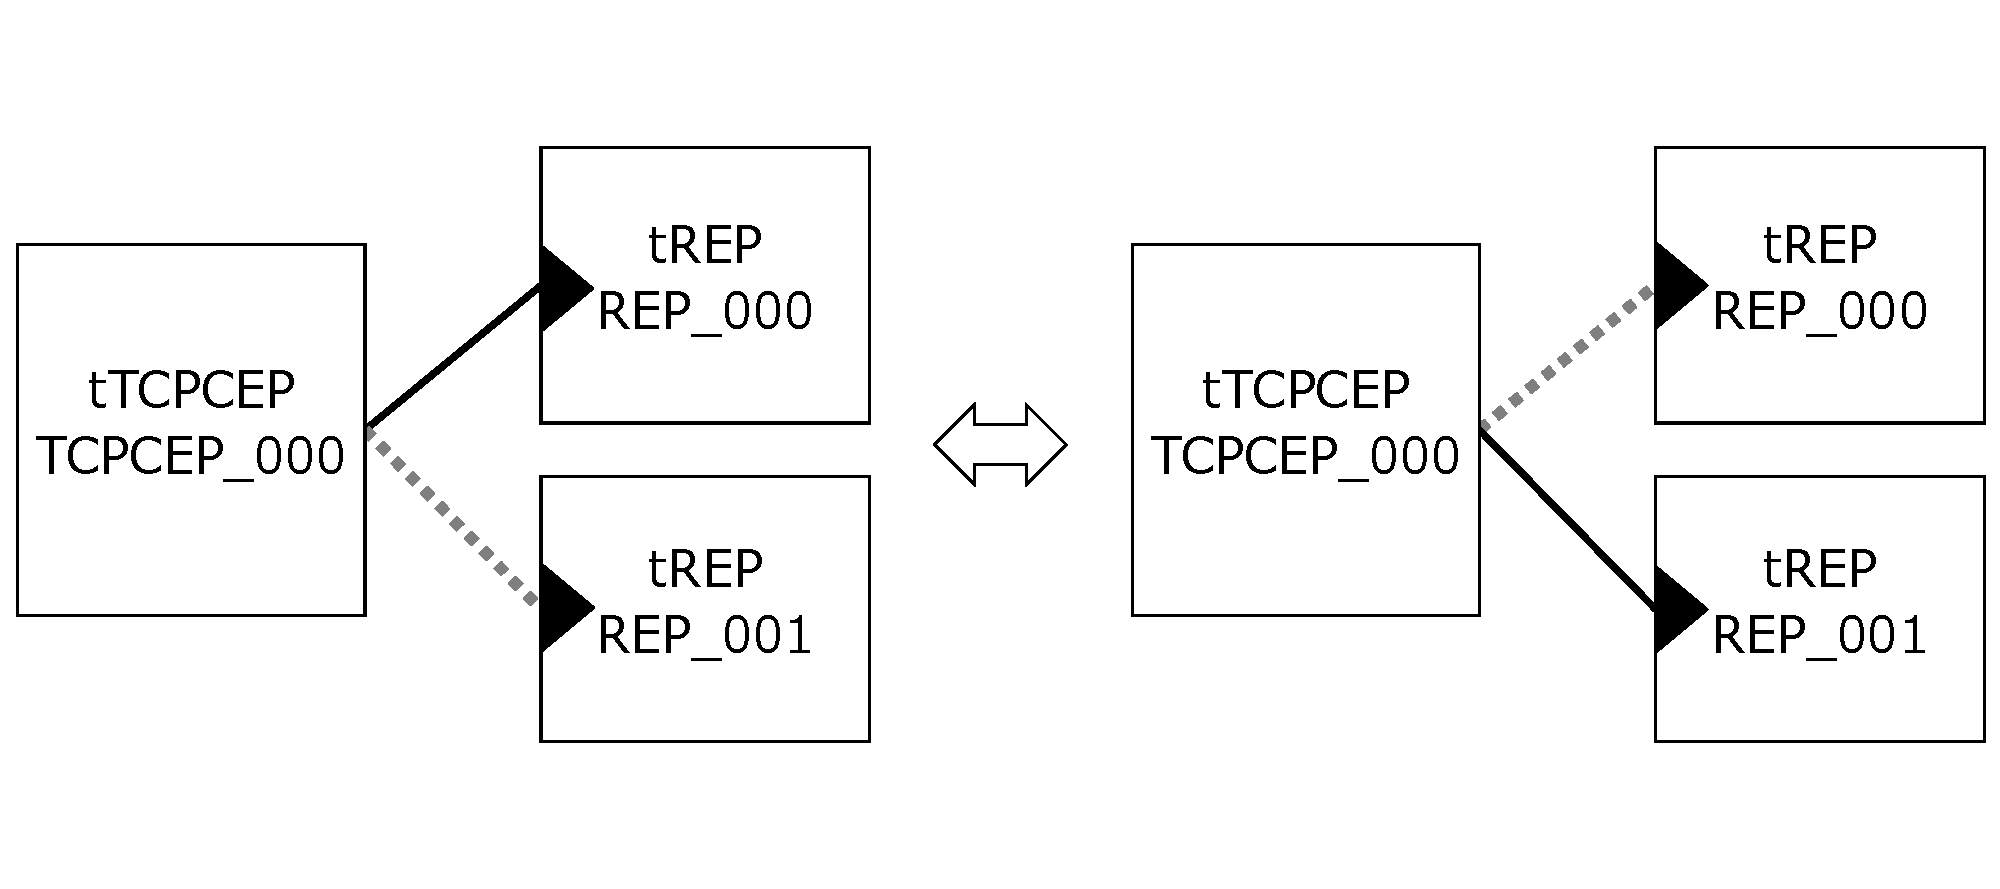
\includegraphics[width=7.0cm,clip]{figure/DynamicConnection.pdf}
    \vspace{-3mm} \caption{Dynamic connection}
    \vspace{-1mm} \label{fig:DynamicConnection}
\end{figure}

TECS supports a dynamic connection, a method for switching the binding of components at runtime (Fig. \ref{fig:DynamicConnection}) as a new functionality.
In Fig. \ref{fig:DynamicConnection}, the solid line represents binding and the dotted line represents non-binding.
Note that all components are statically generated in TECS, which can optimize the overhead of componentization because components are statically configured.
Dynamically generating components causes a good deal of memory consumption, which is a serious problem for embedded systems with strict memory constraints.
The proposed framework can take advantage of the componentization in TINET while satisfying the memory constraint because components are statically generated and dynamically connected in TECS.

TINET+TECS utilizes the dynamic connection to switch between CEP and REP components, as shown in Fig. \ref{fig:DynamicConnectionUseCase}.
In a server application, CEP is associated with REP in the state of waiting for a connection request from clients\footnote{tcp\_acp\_cep(ID cepid, ID repid, T\_IPV4EP *p\_dstaddr, TMO tmout).}.
For example, when processing with the HTTP protocol, CEP passively opens with an REP of port number 80.

\begin{figure}[t]
    \centering
    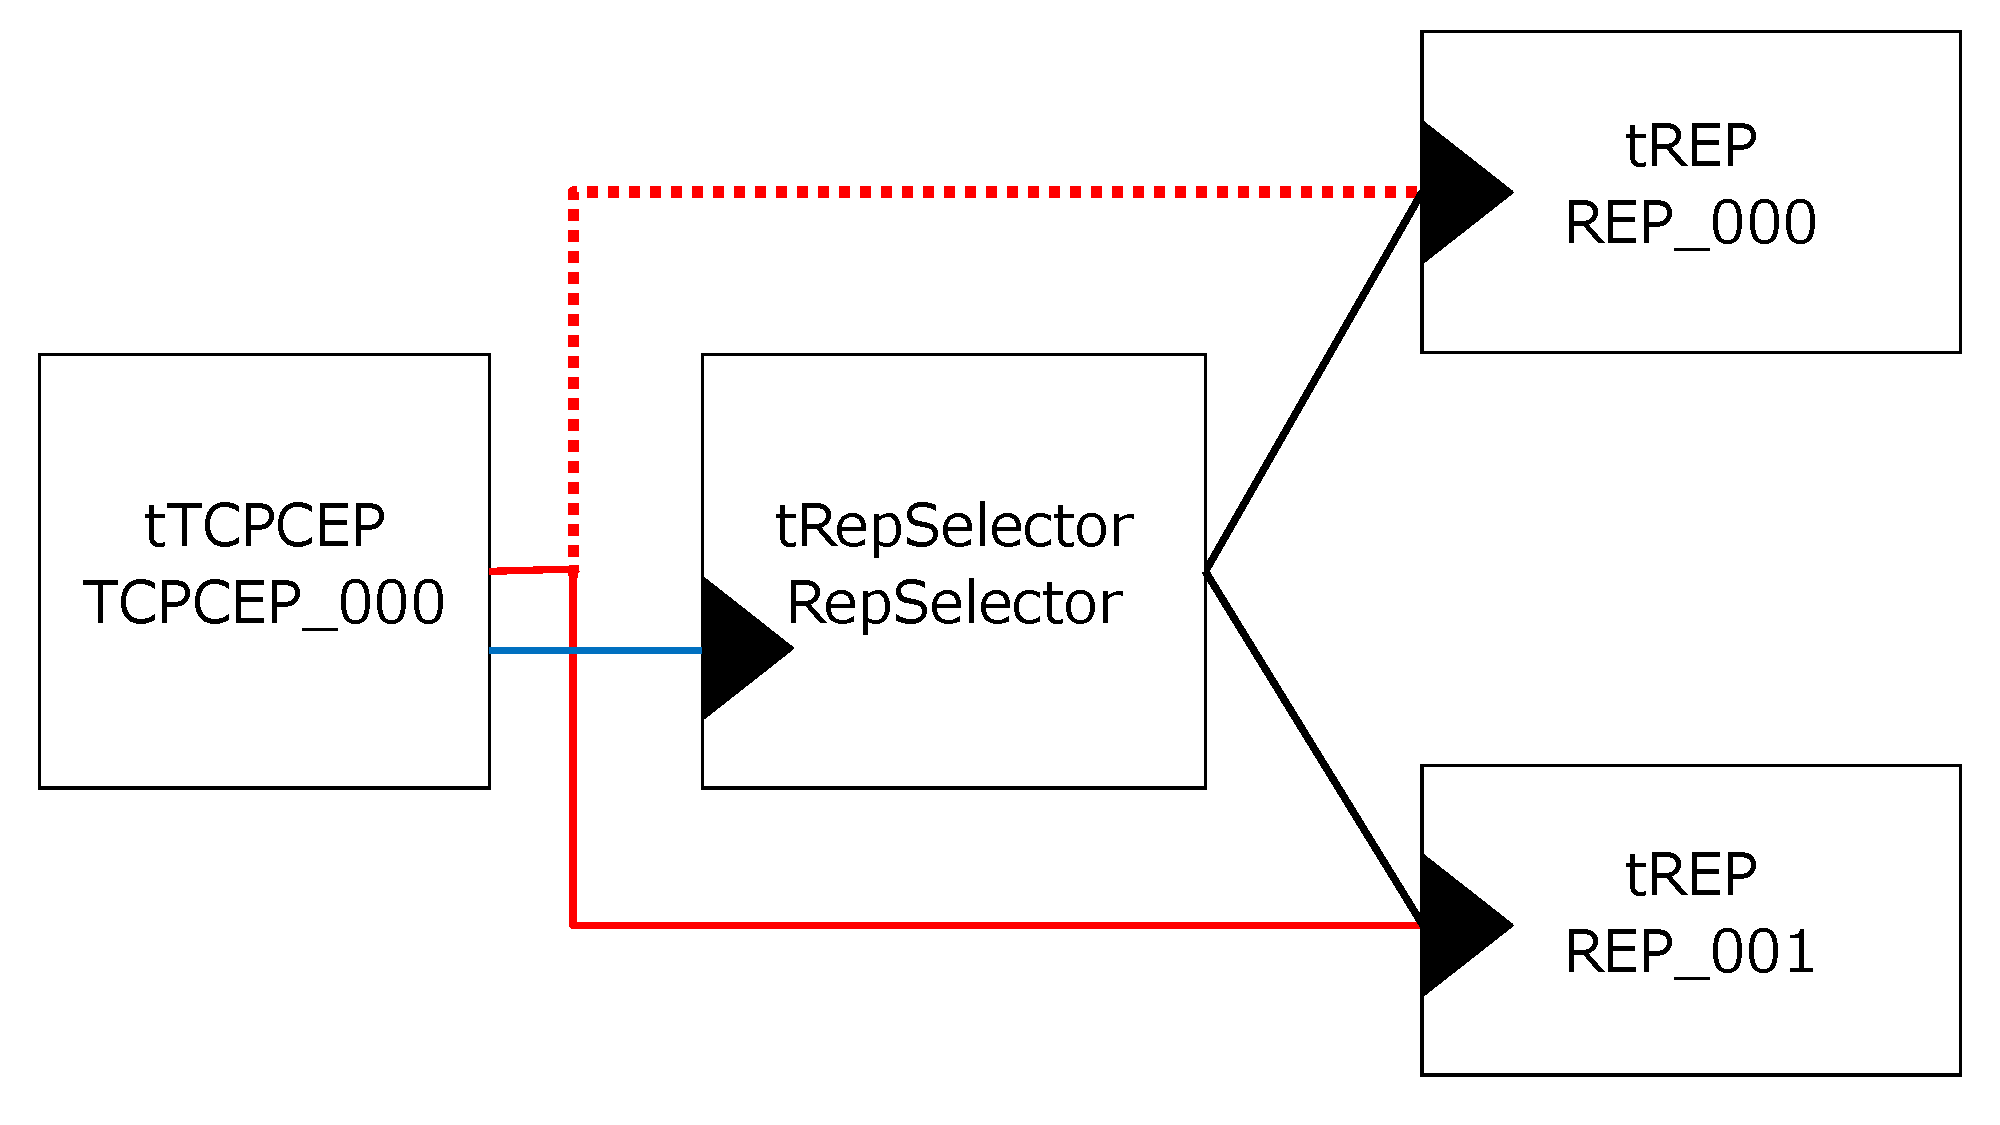
\includegraphics[width=7.0cm,clip]{figure/DynamicConnectionUseCase.pdf}
    \caption{Dynamic connection between CEP and REP}
    \label{fig:DynamicConnectionUseCase}
\end{figure}

To utilize dynamic connectivity, a selector should be defined.
A selector connects all components that can be dynamically connected under a common descriptor that serves as an identifier to access each component \cite{par:optimization}.
The cREP ports form a call port array connecting to connecting to all tREP cells (Line 8 in Fig. \ref{src:DynamicCDLcode}).
{\it [ref\_desc]} is used to identify call ports referring to descriptors. 
In the case shown in Fig. \ref{fig:DynamicConnectionUseCase}, the tRepSelector cell connects all tREP cells.

A CEP component has two call ports: the cRepSelector port, which connects to the eRepSelector port of tRepSelector cell, and the cREP4 port, which connects to either of the tREP cells (Lines 11--13 in Fig. \ref{src:DynamicCDLcode}).
The cREP port is defined using {\it [dynamic]} to identify the call port used to dynamically switch the components.
The call port with the {\it [dynamic]} specifier is not optimized and is allocated in RAM using a plug-in.

\begin{figure}[t]
\centering
\begin{lstlisting}
signature sRepSelector {
    void  getRep([out]Descriptor(sREP4) *desc,
                 [in]int_t i);
};
celltype tRepSelector {
    entry sRepSelector eRepSelector;
    [ref_desc]
        call sREP4 cREP[NUM_REP];
};
celltype tTCPCEP {
    call sRepSelector cRepSelector;
    [dynamic]
        call sREP4 cREP;
    /* Omit: other call/entry ports */
    /* Omit: attributes and variables */
};
\end{lstlisting}
\caption{Signature and celltype description for the dynamic connection}
\label{src:DynamicCDLcode}
\end{figure}

Fig. \ref{src:DynamicCcode} shows a sample code of the dynamic connection.
The eAPI\_accept function is the function wrapping {\it tcp\_acp\_cep} under TECS, which is set as the state waiting for a connection request.
The dynamic connection in the function is performed as shown in Fig. \ref{src:DynamicCcode}.
First, the descriptor of REP to be joined is obtained (Line 3 in Fig. \ref{src:DynamicCcode}).
The first argument, {\it \&desc}, is a variable used to store the descriptor information, whereas the second argument, {\it repid}, is the index of tREP cells.
Next, the descriptor is set (Line 5 in Fig. \ref{src:DynamicCcode}), and the cREP port combines the tREP cell specified by the descriptor, enabling the tCEP cell to call the function of the tREP cell to be joined (Line 7 in Fig. \ref{src:DynamicCcode}).

\begin{figure}[t]
\centering
\begin{lstlisting}
eAPI_accept (.., ..) {
    /* Get a descriptor of intended REP cell */
    cRepSelector_getRep(&desc, repid);
    /* Set the descriptor */
    cREP_set_descriptor(desc);
    /* Call the function of intended REP cell */
    cREP_getEndpoint();
}
\end{lstlisting}
\caption{Accept function (a dynamic connection example)}
\label{src:DynamicCcode}
\end{figure}

\subsection{TLSF+TECS}
\label{sec:TLSF+TECS}

\subsubsection{TLSF}

TLSF (Two-Level Segregate Fit) memory allocator\cite{par:TLSF}\cite{url:TLSF} is a dynamic memory allocator suitable for the real-time system proposed by M. Masmano et al.
TLSF memory allocator has the following features.
\begin{description}
    \item[Real-time property]\mbox{}\\
        The worst execution time required for allocating and deallocating memory does not depend on the data size.
        TLSF always works with $O(1)$, and it is possible to estimate the response time.
    % \item[Fast speed]\mbox{}\\
    %     In addition to being able to always estimate the worst execution time, TLSF is executed at high speed.
    \item[Efficient memory consumption]\mbox{}\\
        Memory efficiency is improved by suppressing memory fragmentation.
        Various tests have obtained an average fragmentation of less than 15\% and a maximum fragmentation of less than 25\%.
\end{description}


\subsubsection{TLSF Algorithms}

TLSF algorithm classifies memory blocks into two stages and searches for a memory block that is optimal for the requested memory size.
The overview of TLSF algorithm is shown in Fig.\ref{fig:TLSF}.
Consider a case where a request, $malloc(100)$, is called to allocate a memory.
In the first step, it is classified by the most significant bit of the requested memory size.
In this case, since 100 is represented by binary number as 1100100, it is in the range from 64 to 128 from the most significant bit.
In the second step, it is further classified.
In this case, 64 to 128 are divided into 4, and 100 is in the block of 96 to 111.
Free block\footnote{Free block is an available memory block.} in this range is used.

A simple fixed-size memory block allocator results in waste of up to 50\%, but TLSF classifies it finely in two steps, so it is a memory efficient algorithm.
In addition, TLSF searches at the same speed and at high speed, $O(1)$.


\begin{figure}[t]
    \centering
    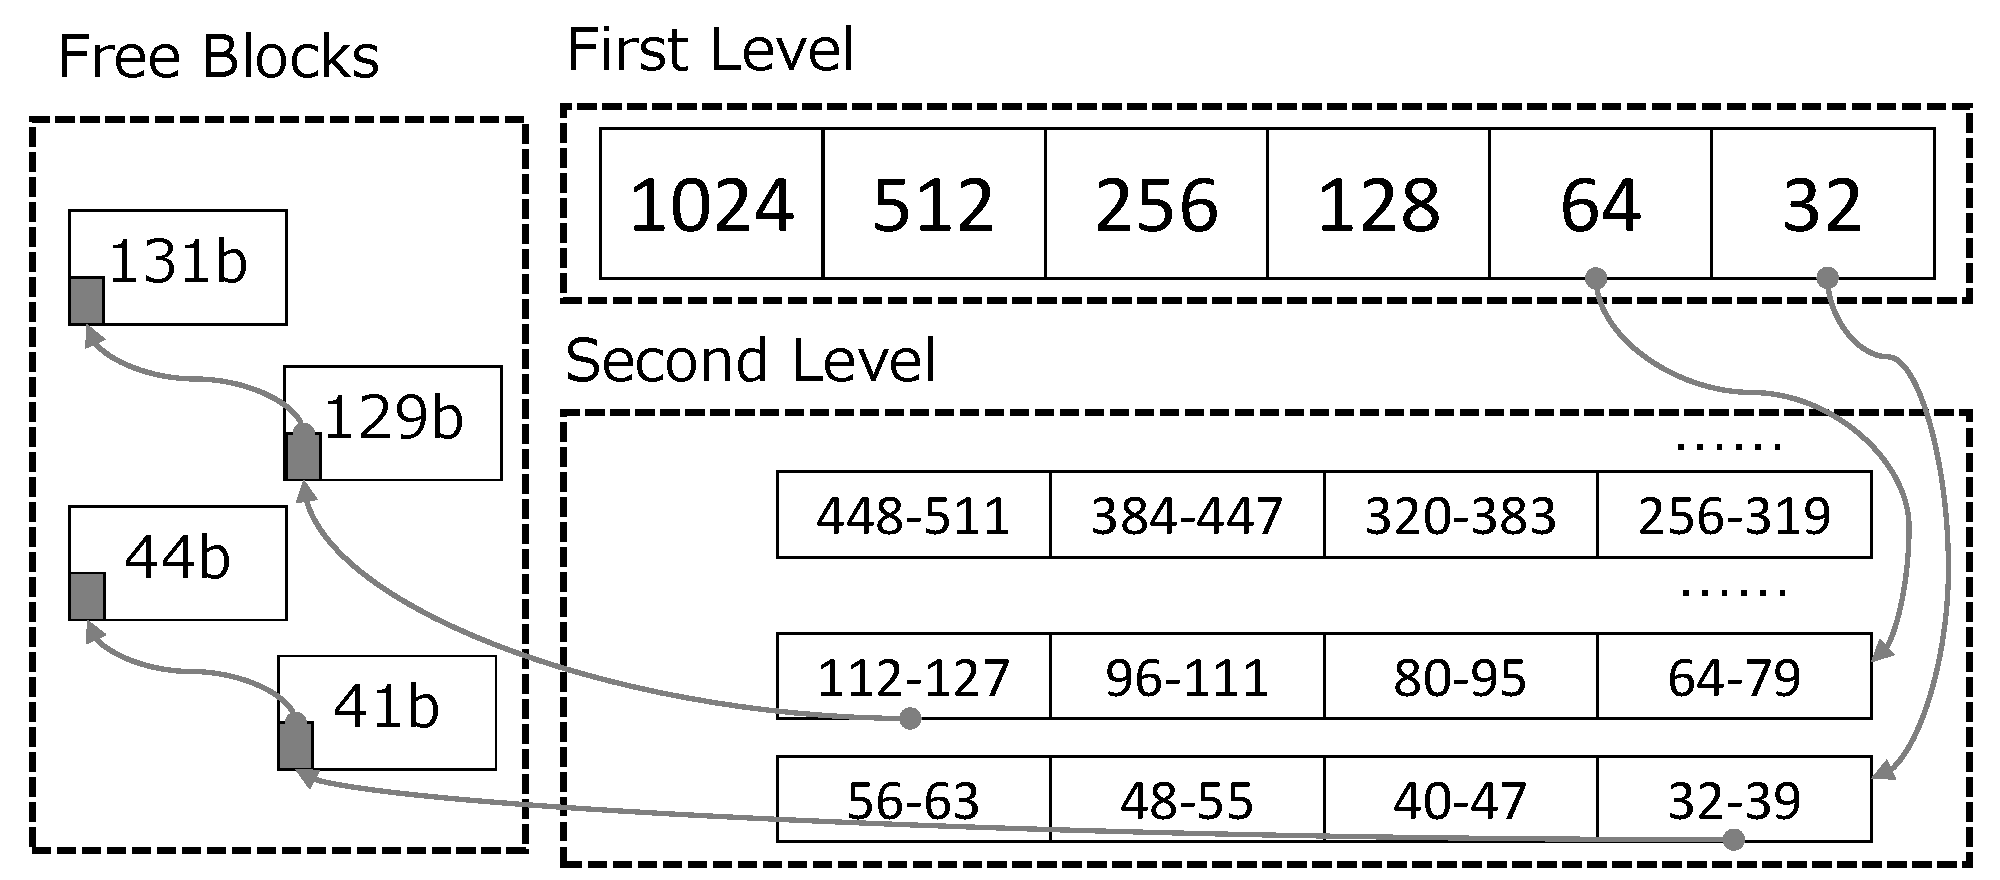
\includegraphics[width=8cm,clip]{figure/TLSF.pdf}
    \caption{TLSF Algorithm}
    \label{fig:TLSF}
\end{figure}


\subsubsection{Component Design of TLSF+TECS}

This section describes the component design of TLSF memory allocator.
In this research, we are using TECS to componentize TLSF.
The version of TLSF used is 2.4.6\footnote{http://www.gii.upv.es/tlsf/main/repo}.

\begin{figure}[t]
\centering
\begin{lstlisting}
signature sMalloc {
    int    initializeMemoryPool(void);
    void   *calloc( [in]size_t nelem,
                    [in]size_t elem_size );
    void   *malloc( [in]size_t size );
    void   *realloc( [in]const void *ptr,
                     [in]size_t new_size );
    void   free( [in]const void *ptr );
};
\end{lstlisting}
\caption{Signature description of memory management}  
\label{src:TLSFSignature}
\end{figure}

Fig.\ref{src:TLSFSignature} is a signature description for memory management used by the allocator.
It defines the memory pool initialization function {\it initializeMemoryPool}, memory allocation function {\it calloc}, {\it malloc}, {\it realloc}, and memory release function {\it free} as a signature.

\begin{figure}[t]
\centering
\begin{lstlisting}
celltype tTLSFMalloc {
    [inline]
        entry  sMalloc  eMalloc;
    attr {
        /* memory pool size in bytes */
        size_t  memoryPoolSize;
    };
    var {
        [size_is( memoryPoolSize / 8 )]
            uint64_t   *pool;
    };
};
\end{lstlisting}
\caption{Celltype description of TLSF memory allocator component}  
\label{src:TLSFCelltype}
\end{figure}

The celltype description of the TLSF memory allocator component is shown in Fig.\ref{src:TLSFCelltype}.
An entry port, {\it eMalloc}, is connected to all components that perform memory management such as $malloc$ and $free$.
Here, {\it [inline]} is a specifier for Implementation as inline functions.
A memory pool size is defined as an attribute, and a pointer to a memory pool is defined as a variable.
Each component holds its own heap area, so even when calling functions for memory management at the same time in different threads, it is possible to operate without memory contention.

\begin{figure}[t]
    \centering
    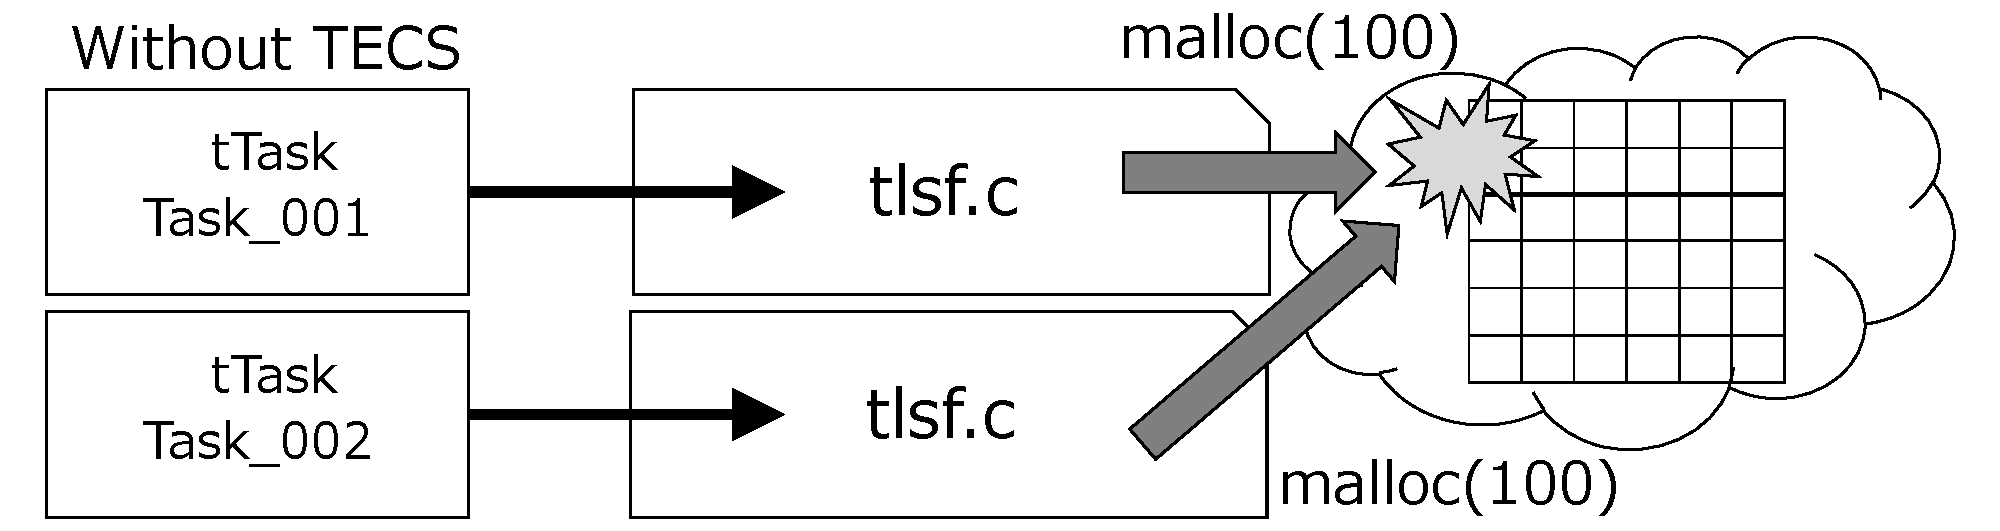
\includegraphics[width=8cm,clip]{figure/WithoutTECS.pdf}
    \caption{TLSF before componentization}
    \label{fig:WithoutTECS}
\end{figure}

\begin{figure}[t]
    \centering
    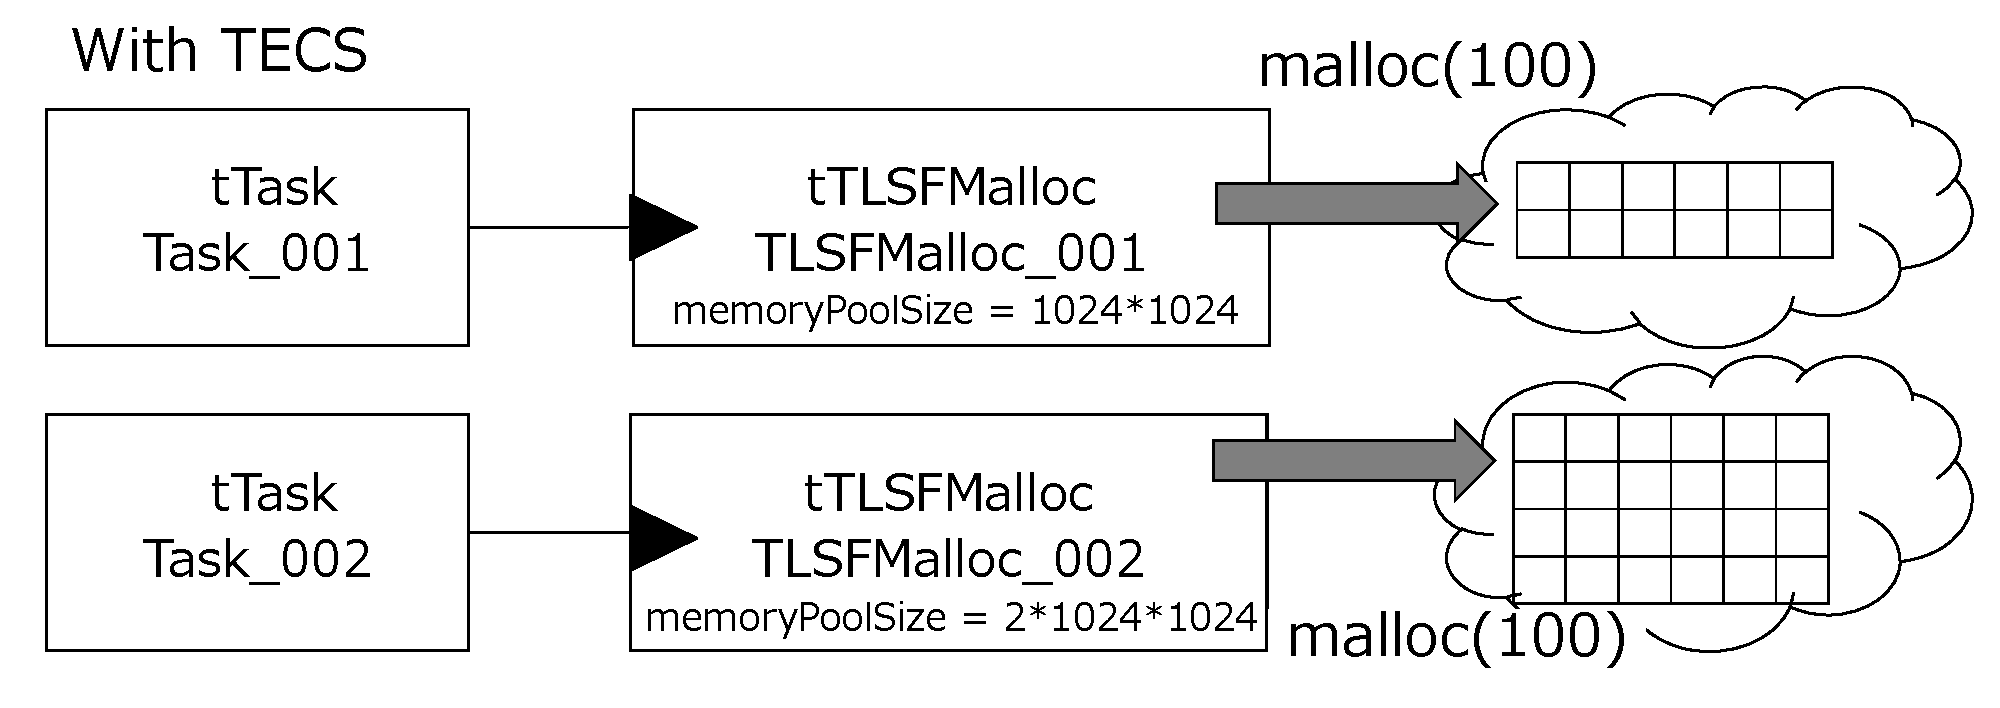
\includegraphics[width=8cm,clip]{figure/WithTECS.pdf}
    \caption{TLSF after componentization}
    \label{fig:WithTECS}
\end{figure}

As shown in Fig.\ref{fig:WithoutTECS}, since TLSF before componentization shares the heap area with multiple threads, if memory is allocated or released simultaneously from multiple threads, memory competition may occur in some cases.
In the research, TLSF is componentized using TECS as shown in Fig.\ref{fig:WithTECS}.
It is possible to operate in thread safe without exclusive control, because each component independently holds a heap area and manages memory within it. 

\begin{figure}[t]
\centering
\begin{lstlisting}
cell tTask Task_001 {
    cMalloc = TLSFMalloc_001.eMalloc;
};
cell tTLSFMalloc TLSFMalloc_001 {
    memoryPoolSize = 1024*1024; /* 1MB */
};
cell tTask Task_002 {
    cMalloc = TLSFMalloc_002.eMalloc;
};
cell tTLSFMalloc TLSFMalloc_002 {
    memoryPoolSize = 2*1024*1024; /* 2MB */
};
\end{lstlisting}
\caption{Build description of TLSF memory allocator component}
\label{src:TLSFBuild}
\end{figure}


\begin{figure}[t]
\centering
\begin{lstlisting}
void*
mrb_TECS_allocf(mrb_state *mrb, void *p, 
                  size_t size, void *ud)
{
    CELLCB	*p_cellcb = (CELLCB *)ud;
    if (size == 0) {
        //tlsf_free(p);
        cMalloc_free(p);
        return NULL;
    }
    else if (p) {
        //return tlsf_realloc(p, size);
        return cMalloc_realloc(p, size);
    }
    else {
        //return tlsf_malloc(size);
        return cMalloc_malloc(size);
    }
}
\end{lstlisting}
\caption{Example of TLSF memory allocator component}  
\label{src:TLSFC}
\end{figure}

Fig.\ref{src:TLSFBuild} shows the build description of the TLSF memory allocator component shown in Fig.\ref{fig:WithTECS}\footnote{Other call/entry ports, attributes, and valuables are actually described, but it is omitted here for the simplicity.}.
Two sets of task components and TLSF components are combined.
Each memory pool size can be configured as a variable (Line 5 and 11 in Fig.\ref{src:TLSFBuild}).
Fig.\ref{src:TLSFC} is the part of the code actually calling the function of the TLSF memory allocator component.
The use part shows a function that the mruby VM allocates memory in the mruby on TECS framework\cite{par:mrubyonTECS}\cite{par:mrubyonTECS3} which is introduced in Section \ref{sec:mrubyonTECS}.
Line 8 calls the {\it free} function of the TLSF memory allocator component.
{\it cMalloc\_} represents the name of the call port (Line 2 in Fig.\ref{src:TLSFBuild}).
Likewise, Line 13 and 17 call the function for memory allocation.
The heap area of {\it TLSFMalloc\_001} component is used if the code of \ref{src:TLSFC} is executed in {\it Task\_001}, and if that is executed in {\it Task\_002}, the heap area of {\it TLSFMalloc\_002} component is used, respectively.
In this way, in the component-based development using TECS, it is possible to operate with the same code without modifying the C code, although the cells are different.

\subsubsection{Multiple RiteVM}

\begin{figure}[t]
    \centering
    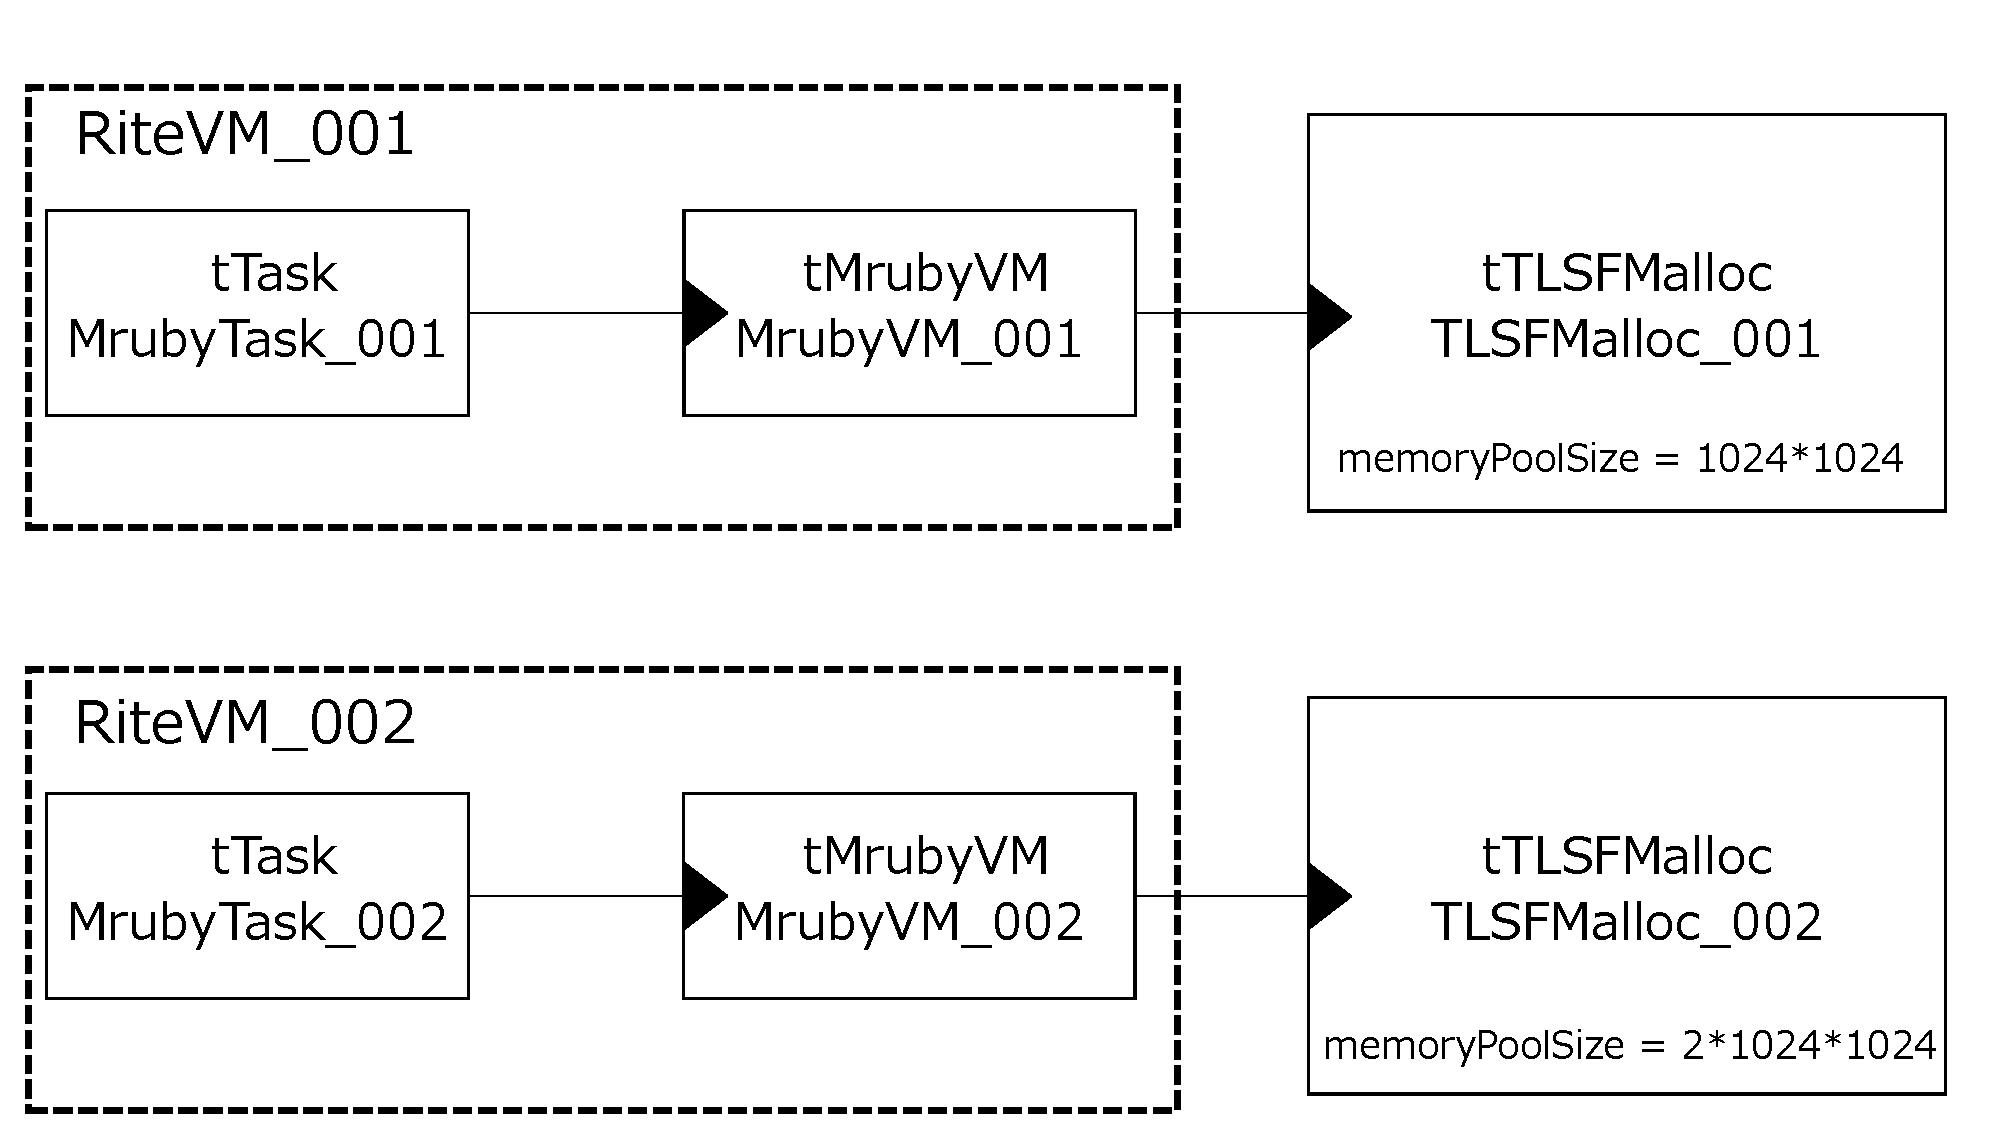
\includegraphics[width=8cm,clip]{figure/UseCase_mruby.pdf}
    \caption{Component description of RiteVM and TLSF+TECS}
    \label{fig:UseCase_mruby}
\end{figure}

The proposed framework uses TLSF memory allocator for memory management of RiteVMs.
However, since the existing TLSF is not thread-safe, if memory is allocated or deallocated from multiple, memory contention will occur.
As a RiteVM allocates and deallocates memory at high frequency, the memory contention immediately occurs in the case of multiple VMs.

The TLSF components are connected to the RiteVMs to hold its own heap area in each RiteVM as shown in Fig.\ref{fig:UseCase_mruby}.
Since each TLSF component holds a memory pool, multiple RiteVMs can be executed without memory contention.
Fig.\ref{fig:UseCase_mruby} shows that the first RiteVM has a heap area of 1 MB (1024*1024) and the second VM has a heap area of 2 MB (2*1024*1024).
It is easy to set different heap areas in each RiteVM.
In addition, RiteVM performs incremental GC (Garbage Collection), and a VM that started GC does not disturb the execution of other VMs by running GC.
    
\subsubsection{Memory management for data sending and receiving}

\begin{figure}[t]
    \centering
    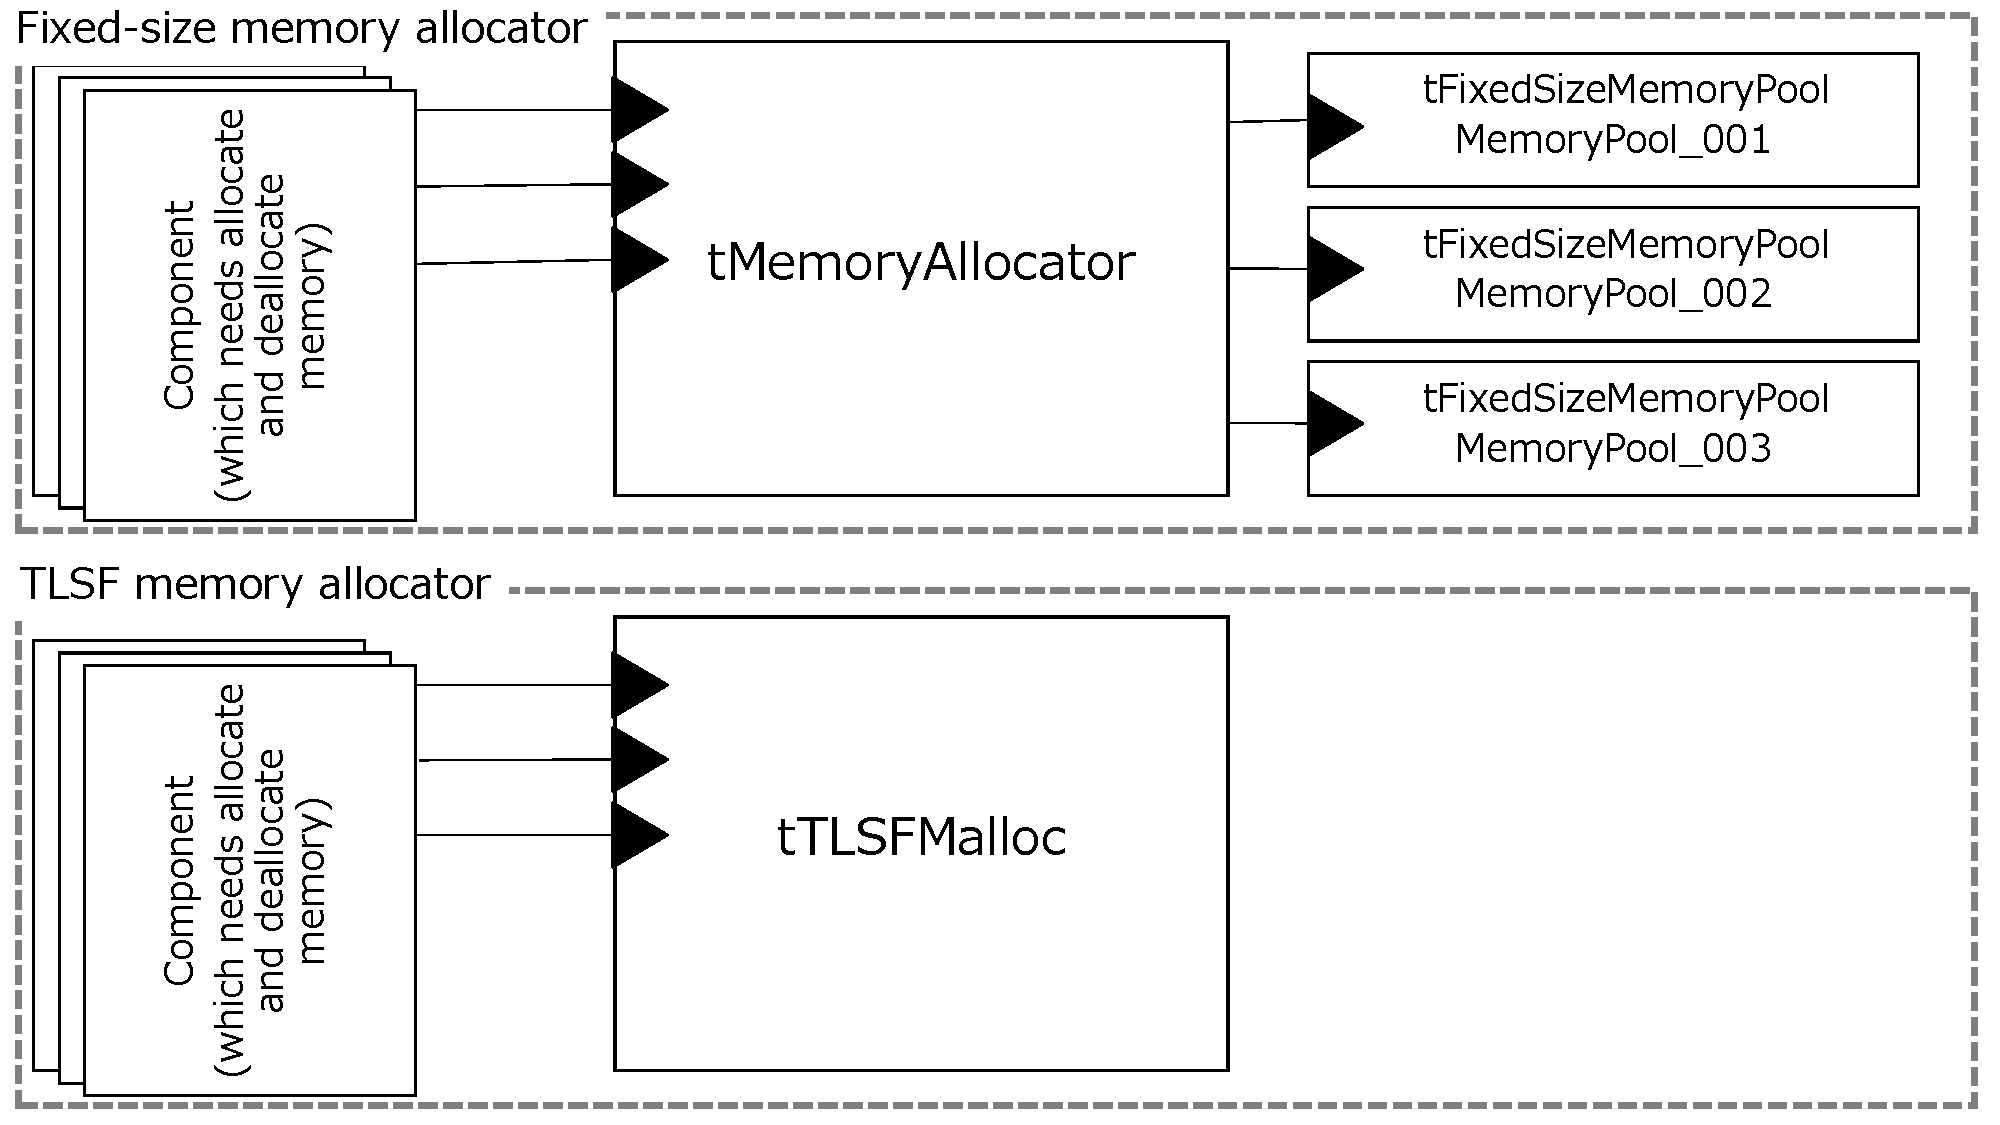
\includegraphics[width=8cm,clip]{figure/UseCase_TINET.pdf}
    \caption{Fixed-size and TLSF memory allocator components}
    \label{fig:UseCase_TINET}
\end{figure}

In TCP/IP protocol stack, memory allocation and release are repeated in each layer such as TCP layer, IP layer, and Ethernet layer, so the role of allocator is important.
TINET+TECS combines all components that manage memory with the allocator.
The TLSF memory allocator can execute at the same speed as compared with the fixed-size memory allocator which TOPPERS/ASP3 supports as standard, and can improve the memory efficiency.
In addition, as shown in Fig.\ref{fig:UseCase_TINET}, the fixed-size memory allocator needs to prepare memory pools of different sizes, and select a memory pool as necessary.
TLSF+TECS efficiently manages the memory without selecting a memory pool.
Since TINET+TECS is component-based system, TLSF+TECS can be easily extended to TINET+TECS.

%4
\subsection{Use case}
\label{sec:UseCase}

In the proposed framework, applications can call TINET functions such as TCP and UDP from mruby programs because mruby-TECS bridge automatically generates the code linking mruby and C.
Fig.\ref{src:mruby} shows an mruby program to transmit the value acquired from a sensor.
mruby makes it easier to develop applications than existing TINET, i.e., C language.

In the case of a simple application, a few functions are only used and there are some unused functions.
For example, the application only uses a function to send by TCP protocol as shown in Fig.\ref{src:mruby}.
The proposed framework incorporates TINET+TECS, and can easily custimize such as removing UDP functions, supporting only IPv4, or removing TCP receiving function.
It can be applied to embedded systems with strict memory constraints by removing unused functions.


\begin{figure}[t]
\centering
\begin{lstlisting}
begin
    io = AnalogIO.new(A0, INPUT)
    cep = TCP.new()	
    cep.accept
    loop do		
        val = io.read  
        cep.snd val.to_s + "\n"		
        RTOS.delay(1000)			
    end
rescue => e	
    puts "[ERROR]" + e
end
\end{lstlisting}
\caption{Example of mruby application}
\label{src:mruby}
\end{figure}


\section{Evaluation}
\label{sec:Evaluation}

This section describes the experimental evaluation used to demonstrate the effectiveness of the proposed framework.

% \subsection{Evaluation environment}

GR-PEACH was employed as the evaluation board.
Detailed specifications of the board are shown in Table \ref{tab:EvaluationBoardEnvironment}.
We also employ TINET 1.5.4 and the compiler arm-none-eabi-gcc 5.2
To pretest the system, we connected the board to a host PC via a LAN cable and evaluated the data sending and receiving.

\begin{table}[t]
    \centering
    \caption{Evaluation Board Environment}
    \begin{tabular}{l|l}
        \hline\hline
        Board           &   GR-PEACH                \\
        CPU             &   Cortex-A9 RZ/A1H 400MHz \\
        Flash ROM       &   8 MB                    \\
        RAM             &   10 MB                   \\
        LAN Controller  &   LAN8710A                \\
        \hline
    \end{tabular}
    \label{tab:EvaluationBoardEnvironment}
\end{table}

\subsection{Performance of TINET+TECS}

To demonstrate the low overhead of TINET+TECS, we compared its execution time and memory consumption with that of TINET, producing the results shown in Fig. \ref{fig:EvaluationOfExecutionTime}.

The {\it tcp\_snd\_dat} and {\it tcp\_rcv\_dat} APIs were used in the evaluation to, respectively, send and receive TCP data.
For {\it tcp\_snd\_dat}, we measured the executing time starting from the API call through the application until the return of the processing result.
In TINET+TECS, this process is performed in the order tApplication, tTCPCEP, tTCPOutputTaskBody, tIPv4Output, tEthernetOutput, tArp, tEthernetOutputTaskBody, and tIfMbed, as shown in Fig. \ref{fig:ComponentProtocolStack}.
For {\it tcp\_rcv\_dat}, we measured the execution time from the data receipt in the LAN driver until data acquisition in the application.
In TINET+TECS, the process is performed in the order tIfMbed, tEthernetInputTaskBody, tIPv4Input, tTCPInput, tTCPCEP, and tApplication, as shown in Fig. \ref{fig:ComponentProtocolStack}.
The execution time of TINET+TECS is close to that of TINET, with an overhead of about 3 us.
As the use of the {\it send/receive} specifier enables accessing of the buffer address without data copying, the componentization overhead does not affect the execution time.

\begin{figure}[t]
    \centering
    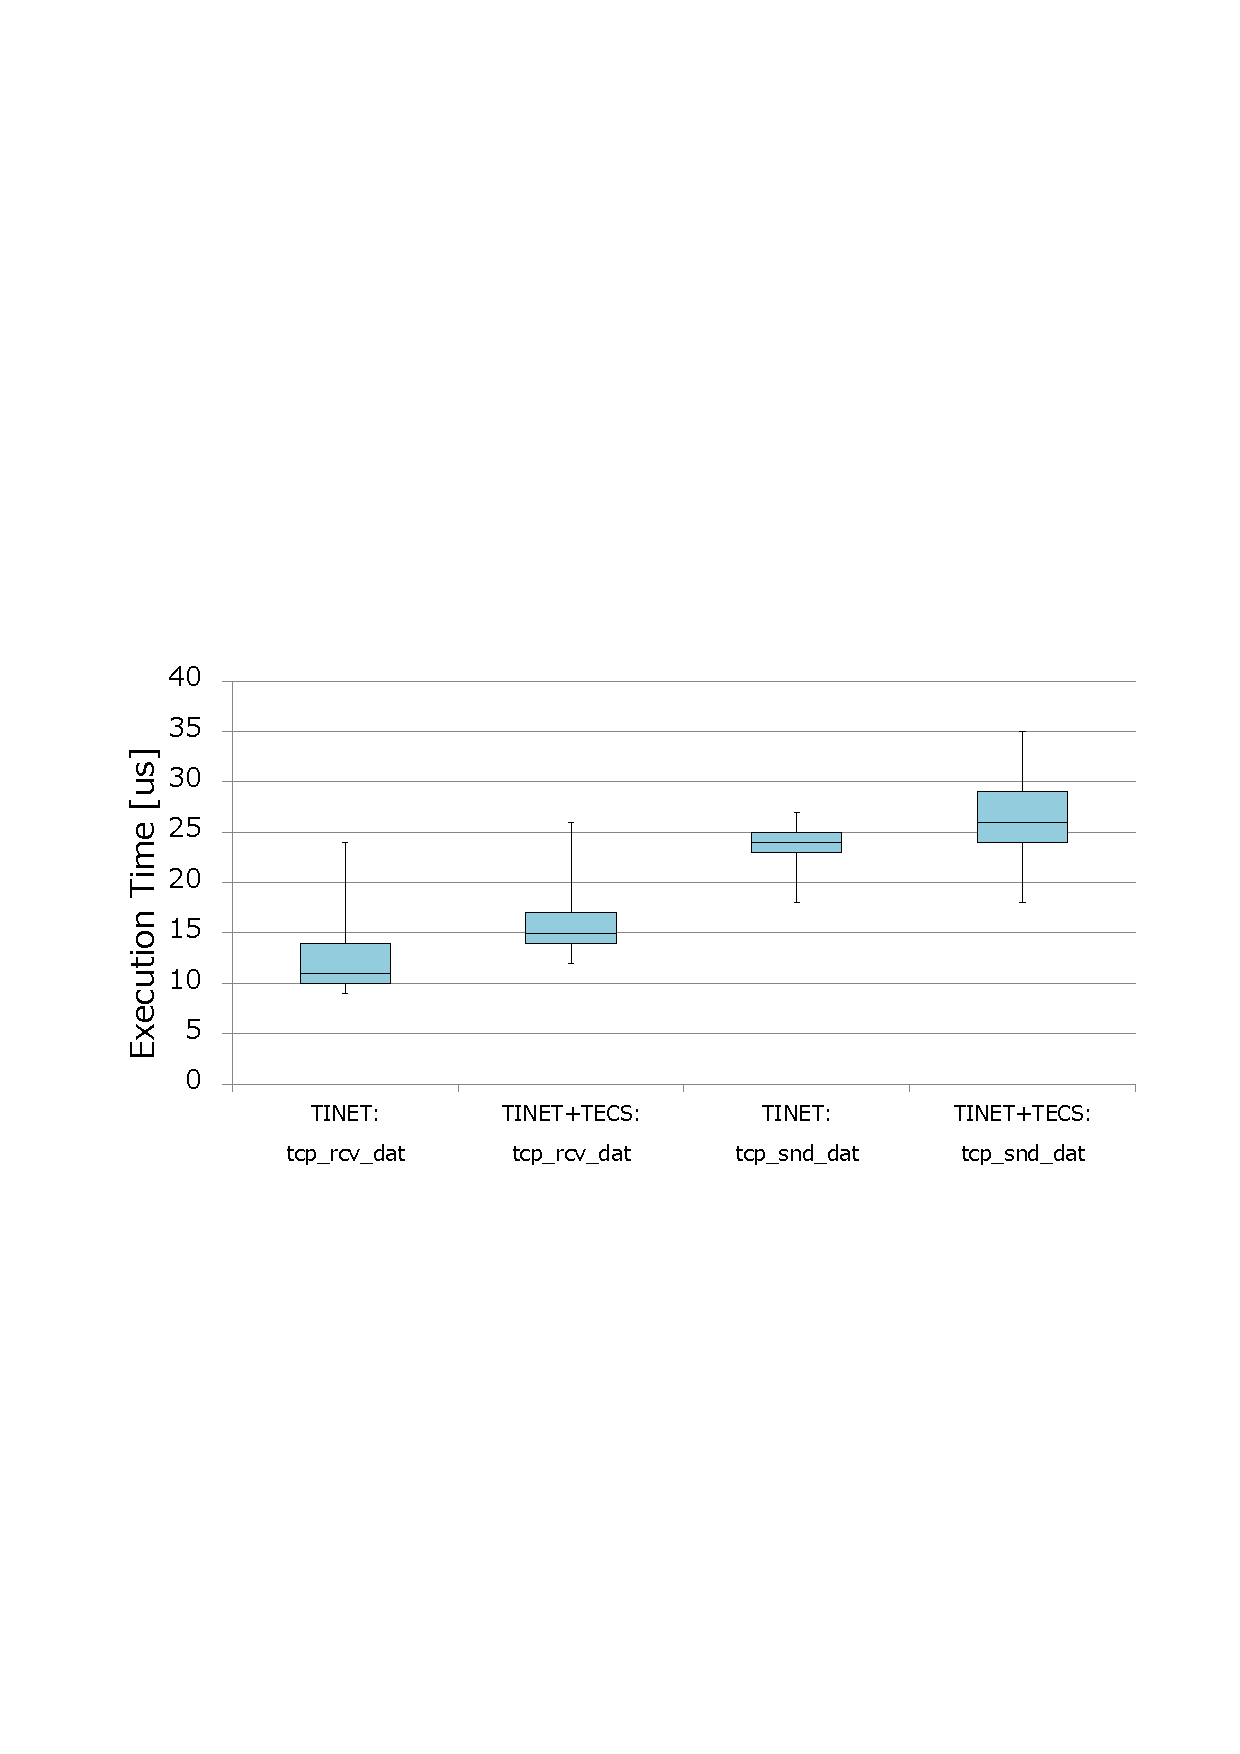
\includegraphics[width=7.5cm,clip]{figure/EvaluationOfExecutionTime.pdf}
    \caption{Execution times of TINET and TINET+TECS}
    \label{fig:EvaluationOfExecutionTime}
\end{figure}

The memory consumptions of TINET and TINET+TECS are compared in Table \ref{tab:EvaluationOfMemoryConsumption}.
The memory consumption of TINET+TECS is about 1\% higher than that of TINET, as the data and processes such as initialization of cells, descriptors, function tables, and skeleton functions needed to manage TECS components increase memory consumption.

\begin{table}[t]
    \centering
    \caption{Memory consumption of TINET and TINET+TECS}
    \begin{tabular}{c|r|r|r|r}
        \hline\hline
                    &   text       &  data    &   bss      &  total     \\ \hline
        TINET       &   183.94 KB  &  5.37 KB &  132.03 KB &  322.34 KB \\
        TINET+TECS  &   170.73 KB  &  5.37 KB &  149.13 KB &  325.23 KB \\
        \hline
        \multicolumn{5}{r}{Including the application and kernel objects}
    \end{tabular}
    \label{tab:EvaluationOfMemoryConsumption}
\end{table}

As shown in Table \ref{tab:EvaluationOfConfigurability}, the code lines for modification were measured to demonstrate the improved configurability.
This demonstrated the ability to change the composition of the protocol stack with a small workload, confirming that the proposed framework improves the configurability.

\begin{table}[t]
    \centering
    \caption{Modified code lines of CDL}
    \begin{tabular}{c|r|r|r}
        \hline\hline
                         &   Size       &   Size (-- Default) & CDL  \\ \hline
        Default          &   325.23 KB  &              0 KB   &  0 lines   \\
        I                &   305.40 KB  &       -- 19.83 KB   & 18 lines   \\
        I + I\hspace{-.1em}I &   304.12 KB  &   -- 21.10 KB   & 27 lines   \\
        I + I\hspace{-.1em}I + I\hspace{-.1em}I\hspace{-.1em}I & 303.45 KB & -- 21.77 KB  & 32 lines \\
        \hline
        \multicolumn{4}{l}{I: Remove TCP}\\
        \multicolumn{4}{l}{I\hspace{-.1em}I: Remove ICMP}\\
        \multicolumn{4}{l}{I\hspace{-.1em}I\hspace{-.1em}I: Change network buffer (Remove memory pools)}
    \end{tabular}
    \label{tab:EvaluationOfConfigurability}
\end{table}

\subsection{Dynamic connection}

\begin{figure}[t]
    \centering
    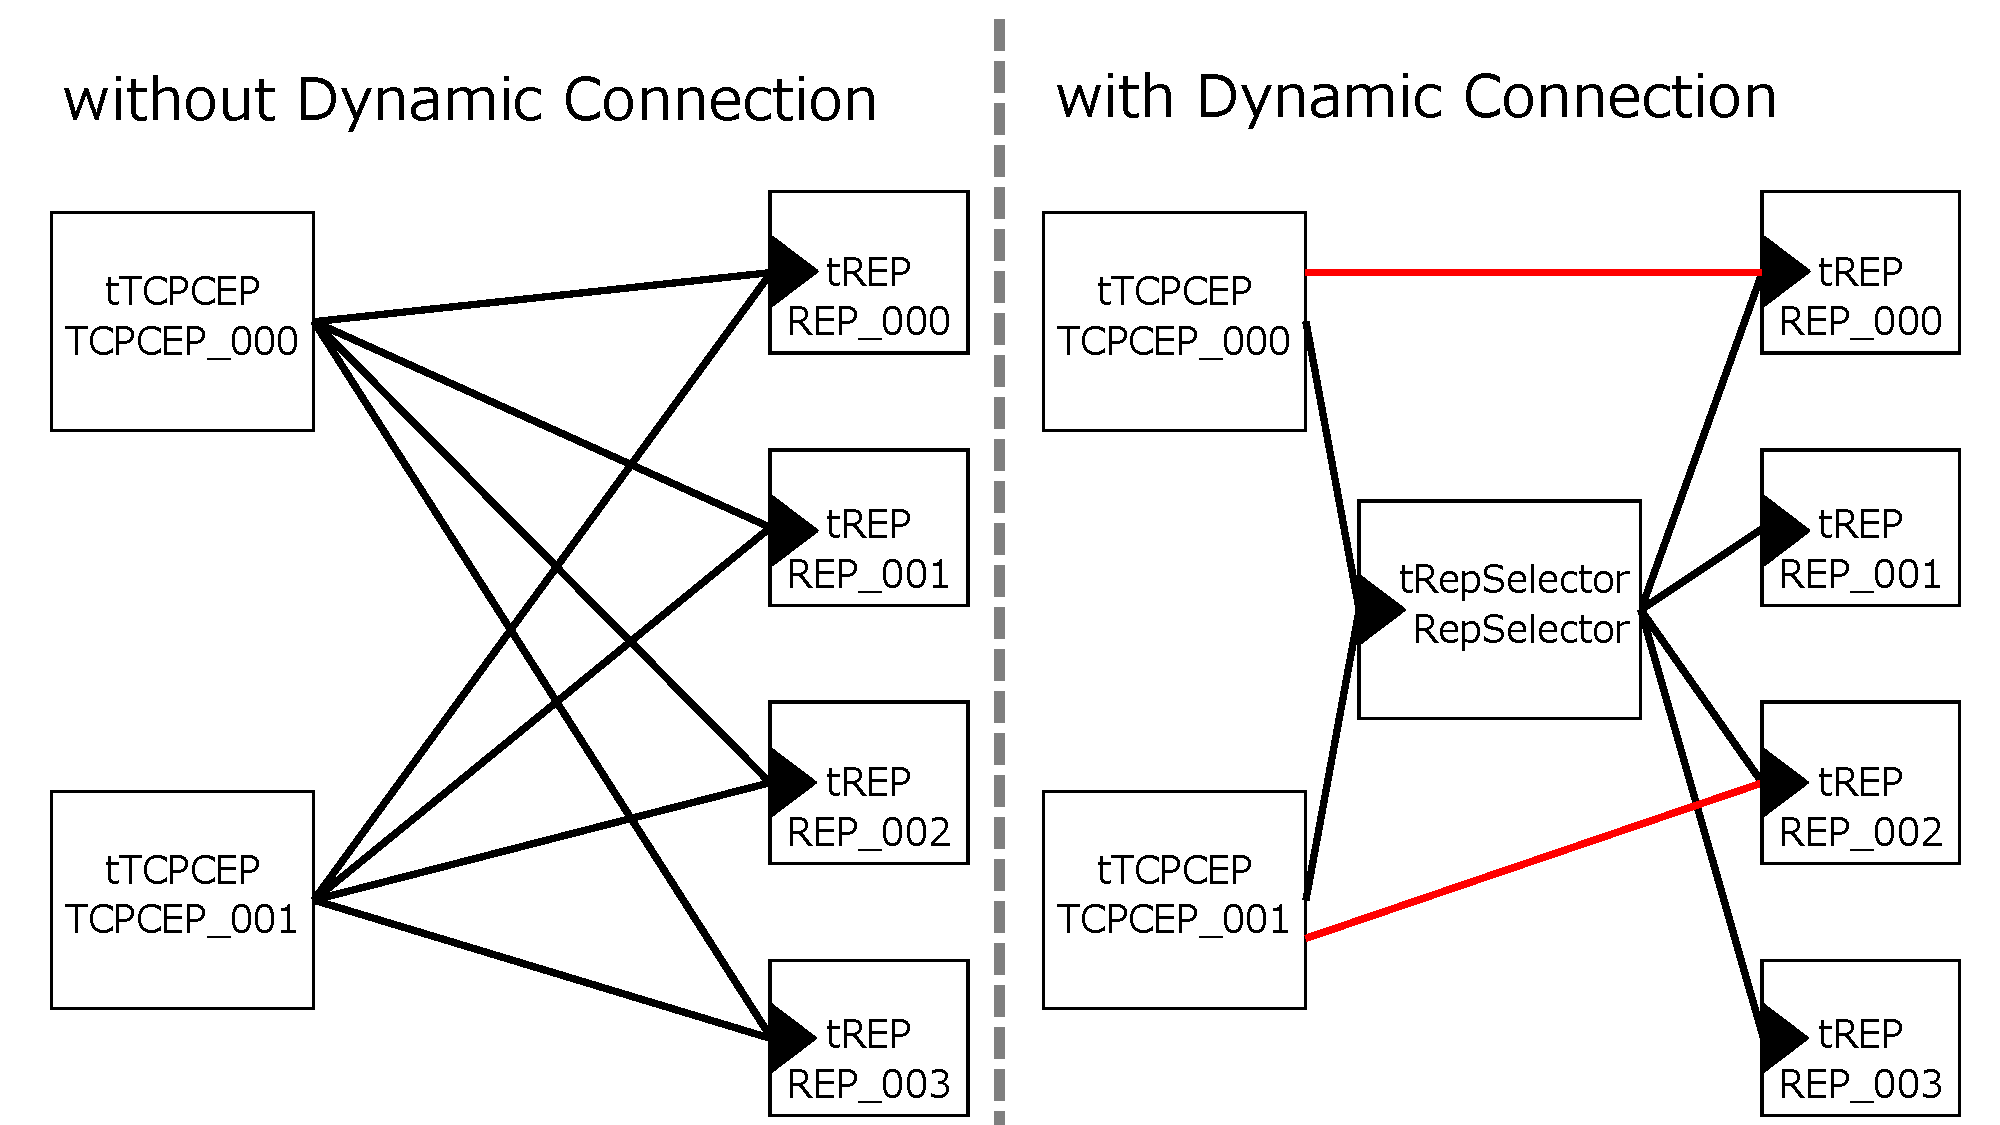
\includegraphics[width=8.0cm,clip]{figure/ComparisonOfDynamicConnection.pdf}
    \vspace{-1mm} \caption{Component diagrams for without/with the dynamic connection cases}
    \vspace{-1mm} \label{fig:ComparisonOfDynamicConnection}
\end{figure}

Memory consumption without and with TECS dynamic connection was then evaluated.
As shown in the left panel of Fig. \ref{fig:ComparisonOfDynamicConnection}, each CEP component should be statically connected to all REP components if the dynamic connection is not used.
As the number of REPs increases, additional call ports of CEP are required, in turn increasing the consumption of memory. 
The dynamic connection reduces memory consumption because only one CEP-to-REP call port is required per CEP, as illustrated with red lines in the right panel of Fig. \ref{fig:ComparisonOfDynamicConnection}.
Even if the number of REPs increases, additional call ports can be joined through the selector, instead of the CEPs.

Memory consumption of without and with dynamic connection is shown in TABLE \ref{fig:EvaluationOfDynamicConnection}.
The dynamic connection case consumes the more RAM memory because, as mentioned in Section \ref{sec:DynamicConnection}, call ports with {\it [dynamic]} are not optimized and allocated in RAM areas.
However, the overall memory consumption is lower under the proposed framework.

% \begin{figure}[t]
%     \centering
%     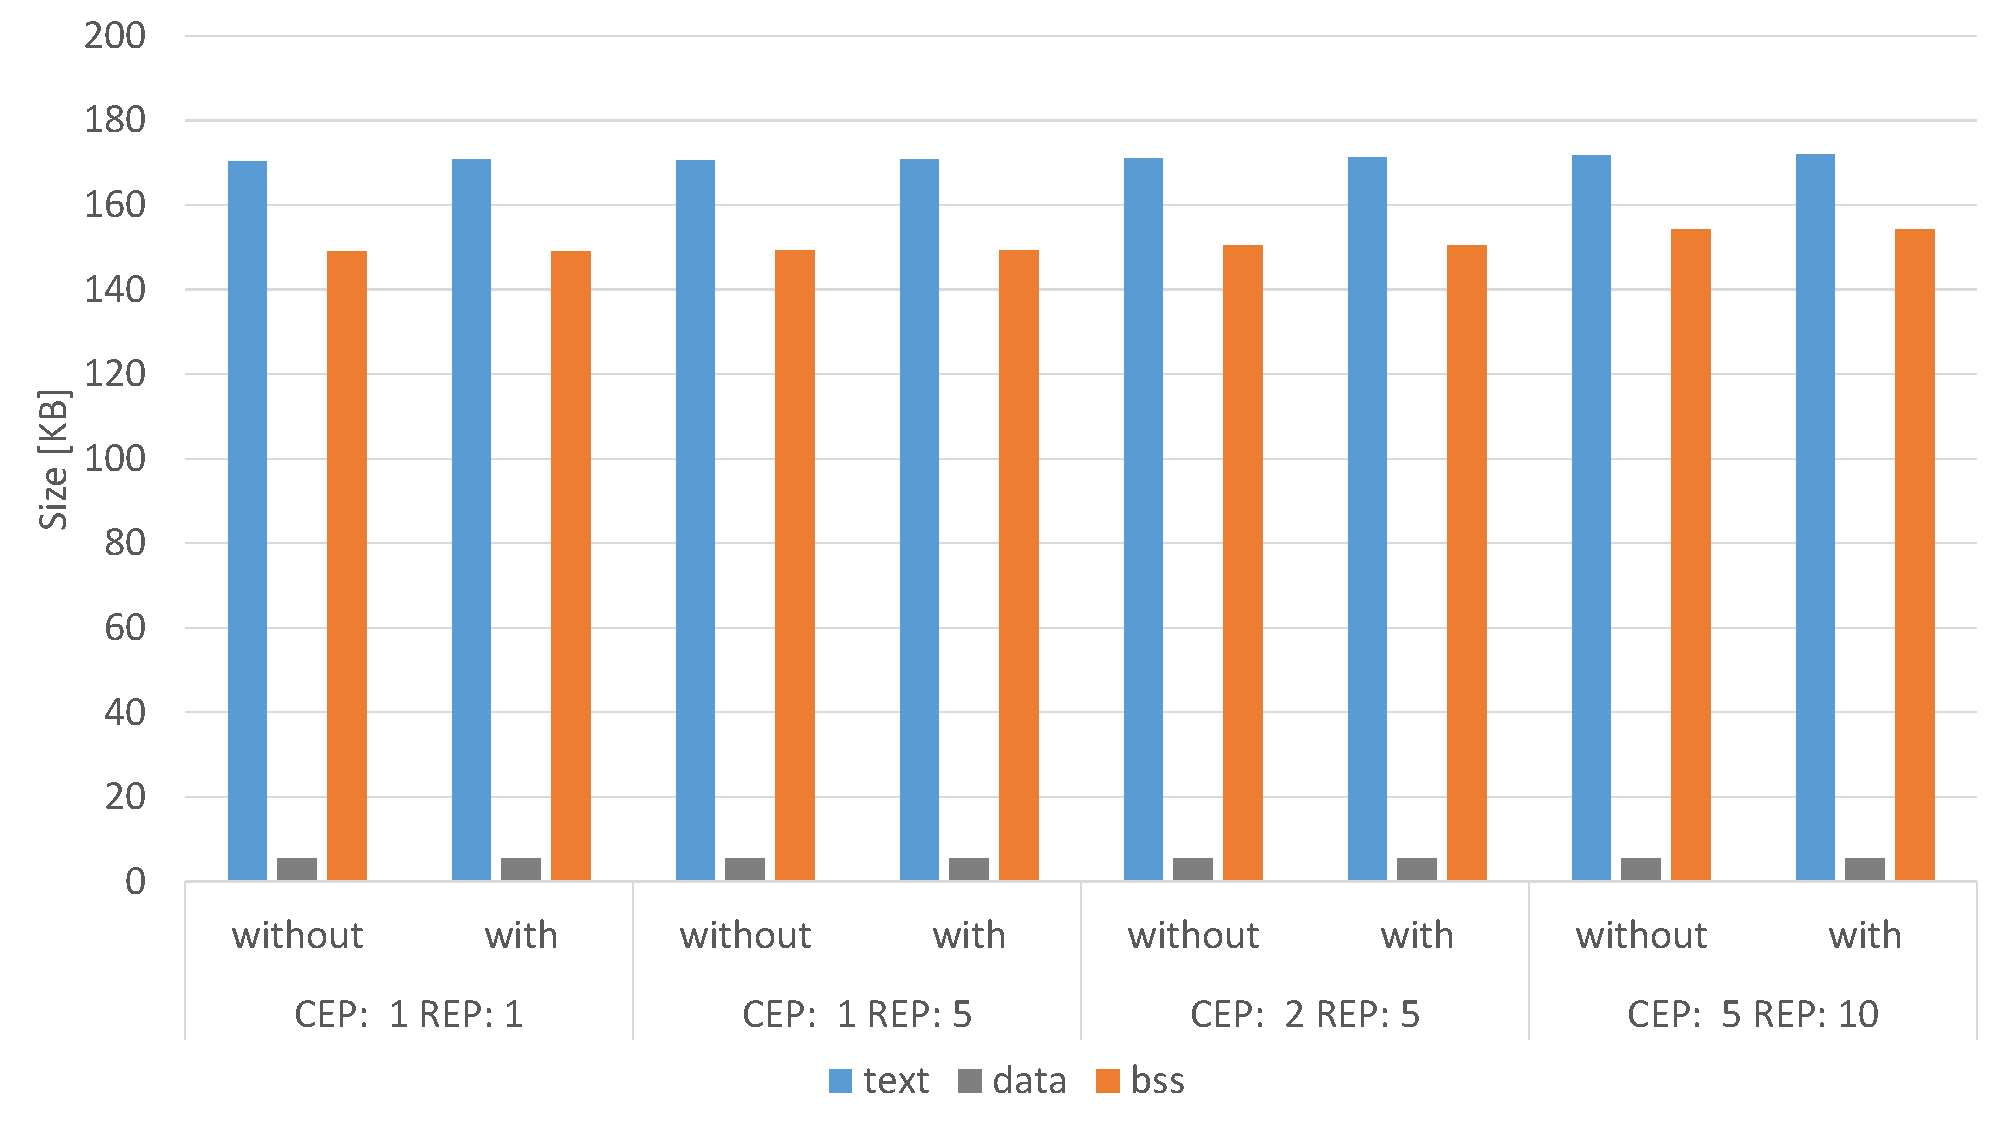
\includegraphics[width=8.0cm,clip]{figure/EvaluationOfDynamicConnection.pdf}
%     \vspace{-1mm} \caption{Memory consumption in two cases (with/without dynamic connection)}
%     \vspace{-1mm} \label{fig:EvaluationOfDynamicConnection}
% \end{figure}
\begin{table}[t]
    \centering
    \caption{Memory consumption in two cases\protect\linebreak (with/without dynamic connection)}
    {\tabcolsep = 1mm
    \begin{tabular}{c|r|r|r|r}
        \hline\hline
                &  CEP:1 REP:1 & CEP:1 REP:5 & CEP:2 REP:5 & CEP:5 REP:10 \\ \hline
        without &  324.98 KB   & 325.34 KB   & 326.39 KB   & 331.68 KB   \\
        with    &  325.23 KB   & 325.32 KB   & 327.24 KB   & 330.48 KB   \\
        \hline
    \end{tabular}
    }
    \label{fig:EvaluationOfDynamicConnection}
\end{table}

\begin{table}[t]
    \centering
    \caption{CDL code lines of without/with dynamic connection}
    \begin{tabular}{l|r|r|r}
        \hline\hline
                     &  without  &  with  &  Diff  \\ \hline
        CEP:1 REP:1  &  344 lines     &  347 lines  &  -3 lines   \\
        CEP:1 REP:5  &  369 lines     &  367 lines  &   2 lines   \\
        CEP:2 REP:5  &  387 lines     &  382 lines  &   5 lines   \\
        CEP:5 REP:10 &  485 lines     &  445 lines  &  40 lines   \\
        \hline
    \end{tabular}
    \label{tab:EvaluationOfConfigurabilityByDynamicConnection}
\end{table}

\begin{figure}[t]
 \centering
 \begin{lstlisting}
/* without Dynamic Connection */
cell tTCPCEP TCPCEP_000 {
    cREP[0] = REP_000.eREP;
    ..
    cREP[n] = REP_00n.eREP;
};
cell tTCPCEP TCPCEP_001 {
    cREP[0] = REP_000.eREP;
    ..
    cREP[n] = REP_00n.eREP;
};
..
cell tTCPCEP TCPCEP_00n {
    cREP[0] = REP_000.eREP;
    ..
    cREP[n] = REP_00n.eREP;
};
 \end{lstlisting}
 \centering
 \begin{lstlisting}
/* with Dynamic Connection */
cell tRepSelector RepSelector {
    cREP[0] = REP_000.eREP;
    ..
    cREP[n] = REP_00n.eREP;
};
cell tTCPCEP TCPCEP_000 {
    cRepSelector = RepSelector.eRepSelector;
};
cell tTCPCEP TCPCEP_001 {
    cRepSelector = RepSelector.eRepSelector;
};
..
cell tTCPCEP TCPCEP_00n {
    cRepSelector = RepSelector.eRepSelector;
};
 \end{lstlisting}
 \caption{Two CDL codes (without/with dynamic connection)}
 \label{src:ComparisonOfCDL}
\end{figure}

The code lines in CDL of without and with the dynamic connection is shown in TABLE \ref{tab:EvaluationOfConfigurabilityByDynamicConnection} to demonstrate improved configurability.
As the number of CEPs and REPs increases, the amount of CDL code lines to be added increases.
In the left panel of Fig. \ref{fig:ComparisonOfDynamicConnection}, each CEP connects all REPs as shown in the upper of Fig. \ref{src:ComparisonOfCDL}. 
In the right panel of Fig. \ref{fig:ComparisonOfDynamicConnection}, a CEP dynamically connects an REP, and only the selector connects all REPs as shown in the lower of Fig. \ref{src:ComparisonOfCDL}. 
It is effective for software that uses many ports because the difference spreads as the number of CEPs and REPs increases.

\subsection{Performance of TLSF+TECS}


%5
\section{Related Work}
\label{sec:Related Work}

To develop the software of IoT systems, several approaches have been proposed \cite{par:frameworkCPS} such as General-purpose Programming Languages (GPLs), Wireless Sensor Network (WSN) macroprogramming, Cloud-based platforms, and Model-Driven Development (MDD).

The development using GPLs such as C, JavaScript, Python, and Android allows the extremely efficient systems based on the complete control over individual devices.
However, GPLs need more development effort, and it is difficult to reuse software due to platform-dependent design.

WSN macroprogramming provides abstractions to specify high-level collaborative behaviors, while hiding low-level details such as message passing and state maintenance.
nesC, a programming language used to build applications for the TinyOS platform \cite{par:nesc}, has been proposed.
nesC/TinyOS is designed for WSN nodes with limited resources e.g., 8 kilobytes of program memory, 512 bytes of RAM, but not supported TCP/IP implementation.

Cloud-based platform reduces development efforts by providing cloud-base APIs and high-level constructs (e.g., drag-and-drop).
In addition, it offers the ease deployment and evolution because the application logic is centrally located in a cloud platform.
However, it is platform-dependent design, and restricts developers in terms of functionality such as in-network aggregation or direct node-to-node communication locally.

To address the issues of development efforts and platform-dependent design, MDD has been proposed \cite{par:MDD}.
MDD provides the benefits of re-usable, platform-independent, extensible design, however it needs long development time to build a MDD system.


%6
\section{Conclusion}
\label{sec:Conclusion}

This paper presented an extended framework of mruby on TECS, including TINET+TECS and TLSF+TECS.
In the proposed framework, mruby programs can call TINET+TECS functions through the mruby-TECS brigde.
Development of software for IoT devices such as sensors and actuators will be more efficient due to the high productivity of mruby.
TINET+TECS is a componentized version of TINET, a compact TCP/IP protocol stack that uses TECS.
It improves on TINET's configurability while suppressing the overhead of componentization.
Scalability is also improved because the component-based framework simplifies to add/remove and change protocols such as TCP/UDP, IPv4/IPv6, and Ethernet/PPP.
This paper also presented the dynamic connection, a new TECS method, to enable dynamic processing while reducing memory consumption.
TINET+TECS utilizes the dynamic connection to satisfy the TINET specification for supporting the static generation of CEPs and REPs.
TLSF+TECS is a component-based dynamic allocator.
Since the TLSF+TECS can hold own heap area, memory contention will not occur even if memory is simultaneously allocated or released from multiple threads.
The heap size can be easily changed because it is set as a variable of the component.
In addition, the RiteVMs, TLSF+TECS, TLSF+TECS are implemented as components; therefore, developers can add, remove, or reuse their functionalities easily as required.
Note that our prototype system and the application programs used in the performance evaluation are all open-source and can be downloaded from our website \cite{url:TECS}.
In the future, we will support mruby libraries as mrbgems, which is an mruby distribution packaging system.\newline

\begin{acknowledgment}
This work was supported by JSPS KAKENHI Grant Number 15H05305.
The authors would like to thank Hiroaki Nagashima and Kazuaki Tanaka for supporting this research.
\end{acknowledgment}


%Reference
\bibliographystyle{ipsj_v2/UTF8/ipsjunsrt-e}
\bibliography{ref}

% \begin{biography}
% \profile{Taro Joho}{was born in 1970. He received his M.S. degree from
% Johoshori University in 1994.
% He joined
% the Information
% Processing Society of Japan in 1994.
% He is currently an associate professor at
% \mbox{Johoshori} University.
% His research interest is online
% publishing systems. He is a member of the IEEE and ACM\@.}
% %
% \profile{Hanako Shori}{was born in 1960. She received her M.E.\ and
% Ph.D.\ from Johoshori University in 1984 and 1987, respectively. She
% became an associate professor at Gakkai University in 1992 and a
% professor at Johoshori University in 1997. Her current research
% interest is online publishing systems. She received the Kiyasu Kinen
% award in 2010. She is a Board Member of the IPSJ and a member of the
% IEICE, IEEE-CS, and ACM\@.} 
% %
% \profile{Jiro Gakkai}{was born in 1970. He received his M.S.\ degree
% from Johoshori University in 1994 and has been engaged in the
% Information Processing Society of Japan since 1994. His research
% interest is online publishing systems. He is a member of the IEEE and
% ACM\@.}
% %
% \end{biography}

\end{document}
